\documentclass[10pt,twocolumn]{article}

\usepackage[a4paper,margin=1.65cm,columnsep=0.65cm]{geometry}
\usepackage{amsmath,amssymb,mathtools}
\usepackage{booktabs,multirow,longtable,array,tabularx}
\usepackage{graphicx}
\usepackage[dvipsnames,table]{xcolor}
\usepackage{microtype}
\usepackage{enumitem}
\usepackage{algorithm}
\usepackage{algpseudocode}
\usepackage{tikz}
\usetikzlibrary{arrows.meta,positioning,fit,calc,backgrounds}
\usepackage[hidelinks]{hyperref}
\hypersetup{
  pdftitle={ReToGCL: Reliability-Weighted Topology-Conditioned Graph Contrastive Learning for Medical Graph Classification},
  pdfauthor={Anonymous Authors},
  pdfsubject={Graph contrastive learning for medical graph classification},
  pdfkeywords={graph neural networks, graph contrastive learning, medical graphs, reliability, topology}
}

\definecolor{viewblue}{HTML}{DCEAF7}
\definecolor{viewgreen}{HTML}{DFF2E1}
\definecolor{reliabilityorange}{HTML}{FCE7C7}
\definecolor{topologypurple}{HTML}{E8DFF5}
\definecolor{contrastred}{HTML}{F7D9D9}
\definecolor{probegray}{HTML}{E8ECEF}
\definecolor{darkblue}{HTML}{1F4E79}
\definecolor{darkgreen}{HTML}{2D6A4F}

\newcommand{\method}{\textsc{ReToGCL}}
\newcommand{\citeneeded}{\textbf{[CITATION NEEDED]}}
\newcommand{\res}[2]{#1\,$\pm$\,#2}
\newcommand{\notrun}{\textit{Not run}}
\newcommand{\R}{\mathbb{R}}
\newcommand{\norm}[1]{\left\lVert #1\right\rVert}
\newcolumntype{Y}{>{\raggedright\arraybackslash}X}

\title{\textbf{ReToGCL: Reliability-Weighted Topology-Conditioned Graph Contrastive Learning for Medical Graph Classification}}
\author{Anonymous Authors\\Anonymous Institution\\\texttt{anonymous@invalid.example}}
\date{Draft manuscript}

\begin{document}
\maketitle

\begin{abstract}
Medical graph classification must learn from heterogeneous graphs whose node attributes and local structures are not equally trustworthy. Standard graph contrastive learning typically treats two stochastic augmentations as equally valid positives and projects every graph into a single unconstrained geometry. These assumptions are fragile for brain-image patch graphs and molecular graphs: attribute corruption can erase clinically relevant signals, subgraph sampling can destabilize local motifs, and class imbalance can make high accuracy coexist with poor minority-class structure. We introduce \method{}, an end-to-end graph contrastive model that combines three ideas: reliable complementary augmentation, sample--view reliability learning, and topology-conditioned projection. An attribute-masked view and a structure-preserving sampled-subgraph view are encoded by a shared three-layer Graph Isomorphism Network. Node-, edge-, local-closure-, graph-, and depth-scale representations provide agreement, stability, and diversity evidence. Continuous reliability weights fuse rather than discard uncertain observations. A topology-conditioned bottleneck then organizes the fused representation before balanced contrastive learning with in-batch and hard negatives. After 40 self-supervised epochs, frozen representations are evaluated by a 200-epoch linear probe under stratified five-fold cross-validation. Across ADHD-200, BZR, COX2, AIDS, and the 12-task Tox21 benchmark, \method{} obtains accuracies of 66.26, 83.93, 82.01, 99.40, and 92.71\%, respectively. Its NMI/ARI/Macro-F1 are 5.88/9.90/62.86 on ADHD-200, 24.22/37.03/73.10 on BZR, 16.67/29.99/70.08 on COX2, 93.69/97.24/99.05 on AIDS, and 11.44/20.79/60.70 on Tox21. Under one unified project implementation, it strictly exceeds all four five-fold means of 34/35, 34/35, 33/35, 30/35, and 28/35 comparators, respectively. These are descriptive mean comparisons, not claims of statistical significance.
\end{abstract}

\section{Introduction}

Graphs provide a common language for biomedical systems. A brain image can be represented as a spatial graph of anatomical patches, while a molecule can be represented as atoms connected by chemical bonds. The resulting graph-classification problems nevertheless differ sharply in graph size, feature semantics, class balance, and label completeness. ADHD-200 contains relatively large, fixed-lattice brain graphs; BZR and COX2 contain small and imbalanced molecular datasets; AIDS contains a pronounced class skew; and Tox21 combines twelve partially observed toxicity endpoints. A representation learner intended for this setting must therefore be robust to both perturbation noise and heterogeneous topology.

Graph contrastive learning (GCL) is attractive because it can pretrain an encoder without diagnostic or activity labels \citeneeded. Most GCL pipelines maximize agreement between two augmented instances of the same graph and use other graphs as negatives. The critical but often implicit assumption is that both augmentations preserve task-relevant information. In medical graphs, that assumption is unreliable. Attribute masking may suppress a localized imaging or chemical signal; subgraph sampling may remove an important motif; and the same corruption strength may be benign for one graph but destructive for another. Uniformly weighting the two views transfers these errors into the contrastive target.

A second difficulty arises after encoding. Ordinary projection heads map all samples into one contrastive geometry. This can place same-class graphs far apart, move boundary samples toward a different class, or obscure a real within-class manifold with high-dimensional noise. These effects are especially consequential under imbalance: accuracy can remain high when a model predominantly predicts the majority class, while Macro-F1, normalized mutual information (NMI), and adjusted Rand index (ARI) expose weak class-balanced separation.

We address these issues with \method{}, a reliability-weighted and topology-conditioned GCL framework. The model constructs complementary attribute-masked and sampled-subgraph views, encodes both using a shared three-layer GIN, and collects evidence at node, edge, local-closure, global-graph, and depth scales. It assigns a continuous reliability distribution to every sample--view pair. Thus, difficult graphs remain in training, but unreliable evidence contributes less. The reliability-fused representation conditions semantic routing and is subsequently organized through a topology-conditioned bottleneck whose structural agreement is regularized. Balanced contrastive learning combines in-batch negatives with representation-dependent hard negatives. The entire pretraining system is optimized jointly, after which a linear classifier evaluates the frozen graph representation.

Our contributions are threefold:

\begin{itemize}[leftmargin=*,nosep]
    \item We formulate reliable complementary augmentation for medical graphs, coupling attribute masking and structure-preserving subgraph sampling without assuming that every perturbed view is equally faithful.
    \item We introduce sample-specific multi-view reliability learning from agreement, cross-augmentation stability, and representation diversity, retaining hard samples through continuous weighting rather than binary rejection.
    \item We combine the reliability mechanism with topology-conditioned projection and balanced contrastive learning in one end-to-end model. Under a unified PyG adaptation, data pipeline, and five-fold protocol, the combination improves medical graph representations across five heterogeneous benchmarks, as jointly assessed by Accuracy, NMI, ARI, and Macro-F1.
\end{itemize}

The empirical statements in this manuscript are deliberately bounded. ``Exceeds'' means that a reported five-fold mean is strictly larger. It does not imply statistical significance, and no significance test is claimed.

\section{Related Work}

\subsection{Graph representation learning in biomedicine}

Message-passing graph neural networks aggregate neighborhood information to form node and graph representations \citeneeded. The Graph Isomorphism Network (GIN) is a widely used expressive backbone for graph classification \citeneeded. Biomedical applications include molecular property prediction, drug activity classification, toxicity screening, and graph-based analysis of neuroimaging data \citeneeded. These applications often combine limited labels with substantial imbalance and structurally heterogeneous samples. Consequently, aggregate accuracy alone is insufficient; class-balanced and clustering-oriented measures are also needed.

\subsection{Graph contrastive learning and augmentation}

GCL learns augmentation-invariant representations by matching multiple views of the same graph \citeneeded. Common transformations include attribute masking, edge dropping, node dropping, and subgraph sampling. A fixed augmentation policy can be brittle because invariance is task- and sample-dependent. Adaptive augmentation methods learn global or instance-dependent perturbations \citeneeded, but many still treat the generated views as equally reliable after they have been produced. \method{} instead evaluates evidence at multiple graph granularities and assigns continuous reliability to each sample--view observation.

\subsection{Reliability, imbalance, and hard negatives}

Noisy views and false negatives can bias a contrastive objective. Reliability estimation, uncertainty weighting, positive refinement, and hard-negative construction have therefore been investigated in self-supervised learning \citeneeded. Class imbalance adds a related failure mode: an embedding can support majority-class accuracy while failing to separate minority examples. BalanceGCL is the direct foundation used in this project and is therefore included explicitly in the main comparison \citeneeded. Our extension preserves balanced positive/negative construction while adding reliable augmentation, multi-view reliability learning, and topology-conditioned projection.

\subsection{Topology-aware graph learning}

Graph topology has been incorporated through motif statistics, higher-order structures, pooling, kernels, topological descriptors, and geometry-aware projection \citeneeded. Local closure patterns are particularly useful because they distinguish tree-like neighborhoods from locally redundant or cyclic structures. However, forcing distinct topological regimes into one projection may distort neighborhood relations. \method{} uses local-closure and depth-scale evidence to condition the projection and explicitly discourages structural distortion.

The comparison pool contains BalanceGCL, HistoGraph, UniImb, DiffLift, MaxCutPool, CellCLAT, DualPrism, KAGNN, MultiNet, HSPGKN, DGDA, RSNN, TopoFormer, and 22 additional methods. Their bibliographic metadata must be verified before submission; all unverified citations are intentionally marked \citeneeded. Importantly, the numerical values reported below are \emph{not} copied from the corresponding papers. They are results of method-specific PyG adaptations run in the same project data pipeline and five-fold evaluation framework.

\section{Problem Definition}

Let a biomedical graph be $G_i=(V_i,E_i,X_i)$, where $V_i$ is the node set, $E_i\subseteq V_i\times V_i$ is the undirected edge set, and $X_i\in\R^{|V_i|\times d_x}$ is the node-feature matrix. A dataset is $\mathcal D=\{(G_i,y_i)\}_{i=1}^{N}$, with a graph label $y_i\in\{1,\ldots,C\}$. During self-supervised pretraining, labels are not used. The learner estimates an encoder $f_\theta$ such that a linear classifier trained on frozen $f_\theta(G)$ separates the downstream classes.

For Tox21, $y_{it}\in\{0,1,\varnothing\}$ denotes the label for endpoint $t\in\{1,\ldots,12\}$. A missing value $\varnothing$ is excluded only from the corresponding endpoint. Each endpoint is split independently with stratification; its four metrics are computed separately, and the final Tox21 result is the unweighted macro-average over endpoints.

The representation problem is to learn a map
\begin{equation}
f_\theta:\mathcal G\rightarrow\R^{d_g}
\end{equation}
that is invariant to semantics-preserving perturbations, sensitive to class-relevant structure, robust to unreliable views, and linearly useful after pretraining. No downstream label enters augmentation, reliability estimation, or contrastive pretraining.

\section{Method}

\subsection{Overview}

Figure~\ref{fig:framework} summarizes \method{}. For each input graph, two complementary perturbations are generated. A shared GIN encodes both views and exposes its layer history. Multi-granularity readouts produce node, edge, local-closure, and graph summaries as well as depth-scale summaries. Cross-view evidence yields a continuous reliability distribution. The fused representation conditions the downstream semantic organization, and a topology-conditioned bottleneck maps it to contrastive space. In-batch and hard negatives enter a balanced objective. All differentiable components are optimized jointly.

\begin{figure*}[t]
\centering
\resizebox{\textwidth}{!}{%
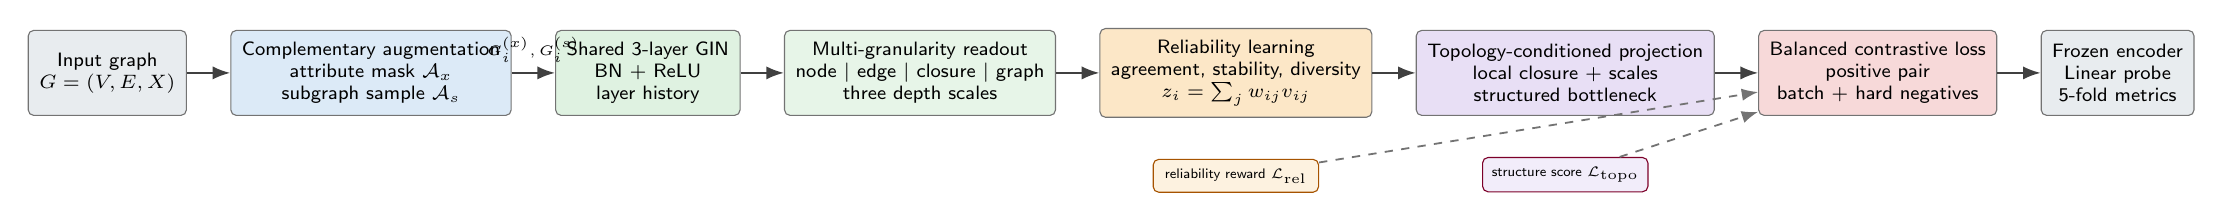
\begin{tikzpicture}[
    font=\sffamily\scriptsize,
    >=Latex,
    stage/.style={draw=black!55, rounded corners=2pt, minimum height=1.08cm, align=center, inner sep=4pt},
    flow/.style={->, line width=0.75pt, draw=black!75},
    aux/.style={->, dashed, line width=0.65pt, draw=black!55},
    note/.style={font=\sffamily\tiny, align=center}
]
\node[stage, fill=probegray, minimum width=1.55cm] (input) {Input graph\\$G=(V,E,X)$};
\node[stage, fill=viewblue, right=0.55cm of input, minimum width=2.15cm] (aug) {Complementary augmentation\\attribute mask $\mathcal A_x$\\subgraph sample $\mathcal A_s$};
\node[stage, fill=viewgreen, right=0.55cm of aug, minimum width=1.90cm] (gin) {Shared 3-layer GIN\\BN $+$ ReLU\\layer history};
\node[stage, fill=viewgreen!75!white, right=0.55cm of gin, minimum width=2.25cm] (multi) {Multi-granularity readout\\node $\mid$ edge $\mid$ closure $\mid$ graph\\three depth scales};
\node[stage, fill=reliabilityorange, right=0.55cm of multi, minimum width=2.25cm] (rel) {Reliability learning\\agreement, stability, diversity\\$z_i=\sum_j w_{ij}v_{ij}$};
\node[stage, fill=topologypurple, right=0.55cm of rel, minimum width=2.25cm] (topo) {Topology-conditioned projection\\local closure $+$ scales\\structured bottleneck};
\node[stage, fill=contrastred, right=0.55cm of topo, minimum width=2.05cm] (cl) {Balanced contrastive loss\\positive pair\\batch $+$ hard negatives};
\node[stage, fill=probegray, right=0.55cm of cl, minimum width=1.75cm] (probe) {Frozen encoder\\Linear probe\\5-fold metrics};

\draw[flow] (input) -- (aug);
\draw[flow] (aug) -- node[above,note] {$G_i^{(x)},G_i^{(s)}$} (gin);
\draw[flow] (gin) -- (multi);
\draw[flow] (multi) -- (rel);
\draw[flow] (rel) -- (topo);
\draw[flow] (topo) -- (cl);
\draw[flow] (cl) -- (probe);

\node[below=0.52cm of rel, draw=orange!65!black, rounded corners=2pt, fill=reliabilityorange!55, note, minimum width=2.1cm] (rreg) {reliability reward $\mathcal L_{\rm rel}$};
\node[below=0.52cm of topo, draw=purple!65!black, rounded corners=2pt, fill=topologypurple!55, note, minimum width=2.1cm] (treg) {structure score $\mathcal L_{\rm topo}$};
\draw[aux] (rreg) -- (cl);
\draw[aux] (treg) -- (cl);
\end{tikzpicture}
}
\caption{End-to-end \method{} framework. The two augmented graphs share every encoder parameter. Continuous reliability weighting retains uncertain samples, while topology-conditioned projection organizes the representation before balanced contrastive learning. The linear probe is trained only after self-supervised pretraining.}
\label{fig:framework}
\end{figure*}

\subsection{Reliable complementary augmentation}

For each $G_i$, we generate
\begin{equation}
G_i^{(x)}=\mathcal A_x(G_i;p_x),\qquad
G_i^{(s)}=\mathcal A_s(G_i;p_s),
\end{equation}
where $\mathcal A_x$ sets selected node-feature vectors to zero and $\mathcal A_s$ retains a density-favored sampled subset while masking removed nodes and incident edges. Both transformations preserve graph identity and enough original content to form a positive pair. Their complementarity is deliberate: the first probes attribute robustness while retaining topology; the second probes structural robustness while retaining the features of selected nodes. In the evaluated configuration, the augmentation budget is 0.10 and the minimum retained-content ratio is 0.60. These values are fixed across the reported runs.

We use the word \emph{reliable} to describe the complete mechanism, not to assert that every generated view is clean. The generator exposes possibly noisy attributes and unstable substructures, after which the reliability module estimates how much each observation should influence training.

\subsection{Shared GIN encoder and multi-layer fusion}

Both views are processed by one parameter-shared three-layer GIN. With $h_v^{(0)}=x_v$, layer $\ell$ computes
\begin{equation}
\label{eq:gin}
\begin{aligned}
h_v^{(\ell)}=\operatorname{ReLU}\!\Bigg(
\operatorname{BN}\!\Bigg[\operatorname{MLP}_{\ell}\!\Bigg(&
(1+\epsilon_{\ell})h_v^{(\ell-1)}\\[-2pt]
&+\sum_{u\in\mathcal N(v)}h_u^{(\ell-1)}\Bigg)\Bigg]\Bigg).
\end{aligned}
\end{equation}
The hidden dimension is 32. We retain $H^{(0)},\ldots,H^{(3)}$ and concatenate sum-pooled layer summaries,
\begin{equation}
g_i=\mathop{\Vert}_{\ell=0}^{3}\operatorname{Pool}\!\left(H_i^{(\ell)}\right),
\end{equation}
which prevents the deepest layer from being the sole source of graph information.

\subsection{Multi-granularity evidence}

Let $\bar h_v$ denote the concatenated node history. Four graph-level views are constructed:
\begin{align}
n_i &= \operatorname{MeanPool}\{\bar h_v:v\in V_i\},\\
e_i &= \operatorname{MeanPool}\{(\bar h_u+\bar h_v)/2:(u,v)\in E_i\},\\
c_i &= \operatorname{MeanPool}\left\{
\frac{|\bar h_v-\mu_{\mathcal N(v)}|}{\sqrt{\deg(v)}}:v\in V_i\right\},\\
g_i &= \operatorname{SumPool}\{\bar h_v:v\in V_i\}.
\end{align}
Here $c_i$ is a differentiable local-closure residual: low residual indicates locally redundant or smoothly closed neighborhoods, whereas high residual exposes unstable or boundary-like structure. Each summary is linearly transformed and $\ell_2$-normalized. In addition, the first, middle, and last GIN states are independently pooled as three depth-scale summaries. Thus, topology and semantics are represented at both granularity and depth axes.

\subsection{Sample--view reliability learning}

For granularity $j\in\{n,e,c,g\}$ and the two augmentations $a\in\{x,s\}$, let $v_{ij}^{(a)}$ be the normalized representation. We calculate
\begin{align}
A_{ij}&=\cos\!\left(v_{ij}^{(x)},v_{ij}^{(s)}\right),\\
S_{ij}&=\exp\!\left[-d_v^{-1}\norm{v_{ij}^{(x)}-v_{ij}^{(s)}}_2^2\right],\\
D_{ij}&=\sqrt{\operatorname{Var}_{k}\left(v_{ij,k}^{(x)}\right)+\varepsilon}.
\end{align}
$A$ measures directional agreement, $S$ measures perturbation stability, and $D$ prevents reliability from collapsing onto an uninformative constant representation. An evidence network produces
\begin{equation}
q_{ij}=\rho_\omega([A_{ij},S_{ij},D_{ij}]),\qquad
w_{ij}=\frac{\exp(q_{ij})}{\sum_{r}\exp(q_{ir})}.
\end{equation}
The reliability-conditioned representations are
\begin{equation}
\label{eq:fusion}
z_i^{(a)}=\sum_jw_{ij}v_{ij}^{(a)}.
\end{equation}
The reliability floor is 0.05 and topology contributes one half of the evidence mixture in the evaluated configuration. Because $w_{ij}$ is continuous and normalized, no sample is removed. The fused representation conditions semantic routing, positive refinement, and hard-negative construction downstream.

We maximize a reliability reward
\begin{equation}
\label{eq:relreward}
\mathcal L_{\mathrm{rel}}=
\frac{1}{B}\sum_{i=1}^{B}\sum_j w_{ij}A_{ij}
+\eta H\!\left(\frac{1}{B}\sum_iw_i\right),
\end{equation}
where the entropy term discourages batch-level collapse onto one granularity. This term is a reward (larger is better), which explains its negative sign in the minimized total objective below.

\subsection{Topology-conditioned representation projection}

Let $t_i$ concatenate the closure view $c_i$ and the three depth-scale summaries. A topology router assigns the graph to a soft mixture of $K$ structural strata,
\begin{equation}
\pi_i=\operatorname{softmax}(R_\psi(t_i)),\qquad
u_i=\sum_{k=1}^{K}\pi_{ik}P_k(z_i),
\end{equation}
where $P_k$ shares a common bottleneck but permits stratum-dependent modulation. The evaluated configuration uses $K=16$, a bridge weight of 0.5, and a 32-dimensional intermediate bottleneck. A learnable projection head maps $u_i$ to the normalized contrastive representation $p_i$.

To preserve topology during organization, define pairwise cosine-distance matrices $\Delta^{\mathrm{topo}}$ from $t$ and $\Delta^{\mathrm{proj}}$ from $p$. We use the topology-preservation score
\begin{equation}
\label{eq:toporeward}
\mathcal L_{\mathrm{topo}}=-\frac{1}{B^2}
\norm{\Delta^{\mathrm{proj}}-\operatorname{sg}(\Delta^{\mathrm{topo}})}_F^2,
\end{equation}
where $\operatorname{sg}$ stops gradients through the evidence target. Since the score is the negative distortion, maximizing it preserves pairwise structure. Conditioning before projection is intended to avoid forcing distinct topology types into an undifferentiated geometry and to reduce the effect of high-dimensional noise on local class structure.

\subsection{Balanced graph contrastive learning}

For graph $i$, the two reliable augmented representations form a positive pair. Other graphs in the minibatch provide negatives, and semantic alternatives generated from non-selected routing prototypes provide hard negatives $h_{ik}^-$. With cosine similarity $s(\cdot,\cdot)$ and temperature $\tau$, one direction of the loss is
\begin{equation}
\begin{aligned}
\ell_i^{x\rightarrow s}
&=-\log\frac{\exp(s(p_i^{(x)},p_i^{(s)})/\tau)}{Z_i},\\
Z_i&=\sum_{r=1}^{B}\exp(s(p_i^{(x)},p_r^{(s)})/\tau)\\[-2pt]
&\quad+\sum_k\exp(s(p_i^{(x)},h_{ik}^-)/\tau).
\end{aligned}
\end{equation}
The contrastive term averages both directions:
\begin{equation}
\mathcal L_{\mathrm{con}}=\frac{1}{2B}\sum_i
(\ell_i^{x\rightarrow s}+\ell_i^{s\rightarrow x}).
\end{equation}
The total minimized objective is
\begin{equation}
\label{eq:total}
\boxed{\mathcal L=
\mathcal L_{\mathrm{con}}
-\lambda_{\mathrm{clean}}\mathcal L_{\mathrm{rel}}
-\lambda_{\mathrm{topo}}\mathcal L_{\mathrm{topo}}.}
\end{equation}
Both auxiliary quantities in Eq.~\eqref{eq:total} are written as rewards. Therefore, the sign convention is equivalent to adding non-negative reliability and topology-distortion penalties. The evaluated implementation uses an auxiliary coefficient of 0.25 per mechanism.

\subsection{Overall formulation and optimization}

Combining Eqs.~\eqref{eq:gin}--\eqref{eq:total}, the end-to-end map is
\begin{equation}
\begin{aligned}
G_i &\xrightarrow{\mathcal A_x,\mathcal A_s}
(G_i^{(x)},G_i^{(s)})
\xrightarrow{f_\theta}
\{v_{ij}^{(a)},t_i^{(a)}\}_{j,a}\\
&\xrightarrow{\rho_\omega}
\{z_i^{(a)}\}_{a}
\xrightarrow{P_{\psi}(\cdot\mid t_i)}
\{p_i^{(a)}\}_{a}
\xrightarrow{\mathcal L}
(\theta,\omega,\psi)^*.
\end{aligned}
\end{equation}
The downstream probe is deliberately excluded from self-supervised optimization.

\begin{algorithm}[t]
\caption{End-to-end pretraining and linear-probe evaluation}
\label{alg:training}
\begin{algorithmic}[1]
\Require Graph dataset $\mathcal D$; encoder $f_\theta$; reliability module $\rho_\omega$; topology-conditioned projector $P_\psi$
\For{$e=1$ to $40$}
    \For{minibatch $\mathcal B\subset\mathcal D$ of size $128$}
        \ForAll{$G_i\in\mathcal B$}
            \State $G_i^{(x)}\gets\mathcal A_x(G_i)$; $G_i^{(s)}\gets\mathcal A_s(G_i)$
            \State Encode both views with the shared three-layer GIN
            \State Read out node, edge, closure, graph, and depth-scale representations
            \State Compute $(A_{ij},S_{ij},D_{ij})$, reliability weights $w_{ij}$, and fused $z_i^{(x)},z_i^{(s)}$
            \State Compute topology evidence $t_i$ and projected $p_i^{(x)},p_i^{(s)}$
        \EndFor
        \State Build in-batch and routing-based hard negatives
        \State Evaluate $\mathcal L_{\rm con}$, $\mathcal L_{\rm rel}$, and $\mathcal L_{\rm topo}$
        \State Update $(\theta,\omega,\psi)$ with Adam on Eq.~\eqref{eq:total}
    \EndFor
\EndFor
\State Freeze $f_{\theta^*}$ and extract graph representations
\For{each stratified fold $k=1,\ldots,5$}
    \State Train a linear classifier for 200 epochs on the fold-training representations
    \State Evaluate Accuracy, NMI, ARI, and Macro-F1 on the held-out fold
\EndFor
\State Report the mean and standard deviation across five folds
\end{algorithmic}
\end{algorithm}

\section{Experimental Setup}

\subsection{Datasets}

Table~\ref{tab:datasets} summarizes the five medical benchmarks. ADHD-200 is a binary structural-MRI graph-classification task. Each subject is represented by a fixed $6\times6\times6$ patch lattice with 216 nodes and 540 undirected edges. Node features contain patch intensity mean, standard deviation, nonzero ratio, and normalized three-dimensional coordinates. The 655 labeled subjects comprise 405 healthy controls and 250 participants with ADHD.

BZR and COX2 are binary molecular-activity datasets. AIDS predicts antiviral activity. Tox21 contains twelve official binary toxicity endpoints. We do not impute missing Tox21 labels; a compound is excluded only for an endpoint whose label is missing. Dataset sources and canonical preprocessing descriptions require bibliographic completion \citeneeded.

\begin{table*}[t]
\centering
\caption{Dataset statistics used in the unified project pipeline. Edge counts are undirected. Tox21 class distributions differ by endpoint and are therefore not summarized as one binary count.}
\label{tab:datasets}
\small
\begin{tabular}{lrrrrrl}
\toprule
Dataset & Graphs & Class distribution & Avg. nodes & Avg. edges & Feature dim. & Task \\
\midrule
ADHD-200 & 655 & 405 / 250 & 216.00 & 540.00 & 6 & ADHD vs. healthy control \\
BZR      & 405 & 319 / 86  & 35.75 & 38.36 & 53 & Benzodiazepine-receptor activity \\
COX2     & 467 & 365 / 102 & 41.22 & 43.45 & 35 & COX-2 inhibitor activity \\
AIDS     & 2,000 & 400 / 1,600 & 15.69 & 16.19 & 38 & HIV/AIDS antiviral activity \\
Tox21    & 7,823 & endpoint-specific & 18.57 & 19.29 & 9 & 12 binary toxicity endpoints \\
\bottomrule
\end{tabular}
\end{table*}

\subsection{Protocol and implementation}

Self-supervised pretraining lasts 40 epochs. The frozen graph encoder is evaluated by a 200-epoch linear probe. We use stratified five-fold cross-validation with random seed 42. The encoder has three GIN layers, hidden dimension 32, ReLU activations, batch normalization, and global pooling. The batch size is 128. Adam uses learning rate $10^{-3}$ and weight decay $10^{-5}$. Every result is reported as the five-fold mean and standard deviation in percentage points.

The protocol is representation evaluation: self-supervised learning uses graph inputs without labels, and each linear probe accesses labels only in its training fold. For Tox21, the split and probe are constructed independently per endpoint, then the endpoint results are macro-averaged. Future work should additionally report a strictly inductive variant that pretrains separately inside each outer fold (Section~\ref{sec:limitations}).

The compared methods share the same project-level PyG interface, processed datasets, split generation, seed, and metric implementation. Their method-appropriate training mechanisms are retained. Consequently, the values in Table~\ref{tab:mainfull} are controlled project reproductions, not numbers directly reported by the cited papers. The archived benchmark contains 35 comparators; the main table shows the 13 requested representative methods and the proposed model, while rank and dominance counts use all 35.

\subsection{Metrics}

Accuracy measures the fraction of correct predictions. Macro-F1 computes F1 independently per class and averages the class values, making it more sensitive to minority-class behavior. NMI measures the mutual dependence between predicted and true partitions after normalization. ARI corrects pairwise partition agreement for chance. For NMI and ARI, hard linear-probe predictions are treated as cluster assignments. Reporting all four prevents majority-class accuracy from being mistaken for uniformly good representation structure.

\section{Main Results}

\subsection{Comparison with unified PyG adaptations}

Table~\ref{tab:mainfull} reports all supplied main-table methods. The proposed row is shaded; this shading denotes the proposed method, not significance. The full 35-method archive is used for ranks in Table~\ref{tab:ranks}.

\onecolumn
\footnotesize
\renewcommand{\arraystretch}{0.80}
\setlength{\tabcolsep}{3pt}
\setlength{\LTleft}{\fill}
\setlength{\LTright}{\fill}
\begin{longtable}{@{}llrrrr@{}}
\caption{Main results under the unified project adaptation and five-fold protocol (mean $\pm$ standard deviation, \%). Values are project reproductions rather than original-paper reports. ``Proposed'' shading identifies \method{}; it does not indicate statistical significance.}
\label{tab:mainfull}\\
\toprule
Dataset & Method & Accuracy & NMI & ARI & Macro-F1 \\
\midrule
\endfirsthead
\multicolumn{6}{c}{\tablename\ \thetable\ --- continued}\\
\toprule
Dataset & Method & Accuracy & NMI & ARI & Macro-F1 \\
\midrule
\endhead
\midrule
\multicolumn{6}{r}{Continued on next page}\\
\endfoot
\bottomrule
\endlastfoot

\multirow{14}{*}{ADHD-200}
& BalanceGCL & \res{62.75}{6.04} & \res{3.78}{5.64} & \res{6.28}{8.20} & \res{58.61}{7.56}\\
& HistoGraph & \res{61.83}{0.00} & \res{0.00}{0.00} & \res{0.00}{0.00} & \res{38.21}{0.00}\\
& UniImb & \res{56.34}{10.29} & \res{0.10}{0.23} & \res{-0.32}{0.71} & \res{36.70}{5.24}\\
& DiffLift & \res{61.53}{0.68} & \res{0.01}{0.03} & \res{-0.10}{0.23} & \res{38.76}{1.23}\\
& MaxCutPool & \res{61.83}{0.00} & \res{0.00}{0.00} & \res{0.00}{0.00} & \res{38.21}{0.00}\\
& CellCLAT & \res{60.46}{3.56} & \res{1.39}{1.74} & \res{2.90}{3.20} & \res{54.31}{3.69}\\
& DualPrism & \res{63.36}{1.95} & \res{1.96}{2.16} & \res{3.65}{3.74} & \res{49.48}{10.66}\\
& KAGNN & \res{61.83}{0.00} & \res{0.00}{0.00} & \res{0.00}{0.00} & \res{38.21}{0.00}\\
& MultiNet & \res{61.83}{0.00} & \res{0.00}{0.00} & \res{0.00}{0.00} & \res{38.21}{0.00}\\
& HSPGKN & \res{62.75}{3.72} & \res{2.91}{2.35} & \res{4.21}{4.69} & \res{53.00}{9.24}\\
& DGDA & \res{62.29}{4.50} & \res{2.58}{2.69} & \res{4.09}{4.55} & \res{53.18}{8.82}\\
& RSNN & \res{61.83}{0.00} & \res{0.00}{0.00} & \res{0.00}{0.00} & \res{38.21}{0.00}\\
& TopoFormer & \res{61.83}{0.00} & \res{0.00}{0.00} & \res{0.00}{0.00} & \res{38.21}{0.00}\\
\rowcolor{topologypurple!45}& \method{} & \res{66.26}{4.23} & \res{5.88}{4.06} & \res{9.90}{5.83} & \res{62.86}{4.55}\\
\midrule

\multirow{14}{*}{BZR}
& BalanceGCL & \res{82.94}{6.90} & \res{21.18}{20.42} & \res{32.91}{23.02} & \res{70.32}{12.42}\\
& HistoGraph & \res{78.77}{0.42} & \res{0.00}{0.00} & \res{0.00}{0.00} & \res{44.06}{0.13}\\
& UniImb & \res{67.16}{25.82} & \res{0.00}{0.00} & \res{0.00}{0.00} & \res{38.70}{11.94}\\
& DiffLift & \res{78.77}{0.42} & \res{0.00}{0.00} & \res{0.00}{0.00} & \res{44.06}{0.13}\\
& MaxCutPool & \res{78.77}{0.42} & \res{0.00}{0.00} & \res{0.00}{0.00} & \res{44.06}{0.13}\\
& CellCLAT & \res{80.73}{4.47} & \res{12.15}{11.89} & \res{20.05}{15.95} & \res{61.97}{10.46}\\
& DualPrism & \res{82.97}{5.63} & \res{16.64}{20.65} & \res{25.20}{25.54} & \res{63.26}{16.16}\\
& KAGNN & \res{78.77}{0.42} & \res{0.00}{0.00} & \res{0.00}{0.00} & \res{44.06}{0.13}\\
& MultiNet & \res{78.77}{0.42} & \res{0.00}{0.00} & \res{0.00}{0.00} & \res{44.06}{0.13}\\
& HSPGKN & \res{78.77}{0.42} & \res{0.00}{0.00} & \res{0.00}{0.00} & \res{44.06}{0.13}\\
& DGDA & \res{77.06}{4.22} & \res{0.03}{0.06} & \res{-0.49}{1.09} & \res{44.82}{1.57}\\
& RSNN & \res{78.77}{0.42} & \res{0.00}{0.00} & \res{0.00}{0.00} & \res{44.06}{0.13}\\
& TopoFormer & \res{78.77}{0.42} & \res{0.00}{0.00} & \res{0.00}{0.00} & \res{44.06}{0.13}\\
\rowcolor{topologypurple!45}& \method{} & \res{83.93}{6.42} & \res{24.22}{18.52} & \res{37.03}{19.92} & \res{73.10}{9.65}\\
\midrule

\multirow{14}{*}{COX2}
& BalanceGCL & \res{83.08}{1.46} & \res{18.23}{4.68} & \res{31.66}{5.09} & \res{70.48}{3.16}\\
& HistoGraph & \res{78.16}{0.46} & \res{0.00}{0.00} & \res{0.00}{0.00} & \res{43.87}{0.14}\\
& UniImb & \res{78.16}{0.46} & \res{0.00}{0.00} & \res{0.00}{0.00} & \res{43.87}{0.14}\\
& DiffLift & \res{78.16}{0.46} & \res{0.00}{0.00} & \res{0.00}{0.00} & \res{43.87}{0.14}\\
& MaxCutPool & \res{78.16}{0.46} & \res{0.00}{0.00} & \res{0.00}{0.00} & \res{43.87}{0.14}\\
& CellCLAT & \res{76.88}{1.51} & \res{0.80}{1.02} & \res{2.93}{3.79} & \res{48.75}{4.08}\\
& DualPrism & \res{78.16}{0.46} & \res{0.00}{0.00} & \res{0.00}{0.00} & \res{43.87}{0.14}\\
& KAGNN & \res{78.16}{0.46} & \res{0.00}{0.00} & \res{0.00}{0.00} & \res{43.87}{0.14}\\
& MultiNet & \res{78.16}{0.46} & \res{0.00}{0.00} & \res{0.00}{0.00} & \res{43.87}{0.14}\\
& HSPGKN & \res{78.16}{0.46} & \res{0.00}{0.00} & \res{0.00}{0.00} & \res{43.87}{0.14}\\
& DGDA & \res{68.05}{22.42} & \res{0.10}{0.23} & \res{0.76}{1.71} & \res{40.61}{7.24}\\
& RSNN & \res{78.16}{0.46} & \res{0.00}{0.00} & \res{0.00}{0.00} & \res{43.87}{0.14}\\
& TopoFormer & \res{78.16}{0.46} & \res{0.00}{0.00} & \res{0.00}{0.00} & \res{43.87}{0.14}\\
\rowcolor{topologypurple!45}& \method{} & \res{82.01}{2.12} & \res{16.67}{5.57} & \res{29.99}{4.00} & \res{70.08}{1.30}\\
\midrule

\multirow{14}{*}{AIDS}
& BalanceGCL & \res{99.45}{0.45} & \res{94.20}{4.37} & \res{97.49}{2.04} & \res{99.14}{0.70}\\
& HistoGraph & \res{93.50}{1.08} & \res{56.47}{5.40} & \res{71.97}{3.92} & \res{89.77}{1.46}\\
& UniImb & \res{96.85}{2.97} & \res{77.68}{14.87} & \res{85.51}{13.92} & \res{94.52}{5.76}\\
& DiffLift & \res{79.75}{0.43} & \res{0.05}{0.09} & \res{-0.15}{0.20} & \res{44.60}{0.38}\\
& MaxCutPool & \res{99.30}{0.27} & \res{92.81}{2.45} & \res{96.79}{1.26} & \res{98.89}{0.44}\\
& CellCLAT & \res{99.30}{0.21} & \res{92.93}{1.71} & \res{96.78}{0.96} & \res{98.89}{0.34}\\
& DualPrism & \res{91.65}{2.00} & \res{48.64}{7.87} & \res{65.48}{7.18} & \res{87.34}{2.81}\\
& KAGNN & \res{92.70}{2.46} & \res{52.76}{11.90} & \res{69.17}{9.89} & \res{88.65}{4.00}\\
& MultiNet & \res{86.65}{5.05} & \res{27.23}{19.28} & \res{39.93}{25.34} & \res{72.42}{16.64}\\
& HSPGKN & \res{96.60}{0.80} & \res{72.62}{5.12} & \res{84.71}{3.63} & \res{94.55}{1.36}\\
& DGDA & \res{92.85}{1.58} & \res{52.26}{7.09} & \res{68.95}{6.77} & \res{88.41}{2.91}\\
& RSNN & \res{99.30}{0.60} & \res{93.37}{5.18} & \res{96.78}{2.75} & \res{98.88}{0.96}\\
& TopoFormer & \res{94.40}{1.01} & \res{61.03}{5.02} & \res{76.06}{4.04} & \res{91.48}{1.51}\\
\rowcolor{topologypurple!45}& \method{} & \res{99.40}{0.28} & \res{93.69}{2.40} & \res{97.24}{1.31} & \res{99.05}{0.46}\\
\midrule

\multirow{14}{*}{Tox21}
& BalanceGCL & \res{92.64}{4.40} & \res{9.41}{11.20} & \res{16.88}{16.70} & \res{58.38}{9.06}\\
& HistoGraph & \res{92.65}{4.65} & \res{9.39}{13.33} & \res{15.59}{20.24} & \res{57.22}{11.42}\\
& UniImb & \res{91.92}{5.36} & \res{1.15}{3.62} & \res{2.65}{7.77} & \res{49.87}{4.93}\\
& DiffLift & \res{92.25}{4.76} & \res{1.68}{4.77} & \res{3.40}{9.15} & \res{50.10}{5.50}\\
& MaxCutPool & \res{92.38}{4.80} & \res{4.63}{10.70} & \res{7.54}{16.92} & \res{52.15}{9.61}\\
& CellCLAT & \res{92.13}{4.77} & \res{2.09}{2.65} & \res{4.74}{5.33} & \res{51.34}{3.11}\\
& DualPrism & \res{92.66}{4.51} & \res{8.67}{12.19} & \res{14.87}{19.21} & \res{56.97}{10.80}\\
& KAGNN & \res{92.50}{4.66} & \res{5.78}{11.09} & \res{9.67}{18.12} & \res{53.49}{10.50}\\
& MultiNet & \res{92.34}{4.83} & \res{3.99}{10.07} & \res{6.41}{15.72} & \res{51.42}{8.93}\\
& HSPGKN & \res{92.38}{4.89} & \res{6.07}{12.05} & \res{10.05}{18.38} & \res{53.85}{10.39}\\
& DGDA & \res{92.54}{4.58} & \res{7.14}{11.29} & \res{11.81}{18.25} & \res{54.90}{10.42}\\
& RSNN & \res{92.67}{4.56} & \res{7.99}{12.33} & \res{12.94}{19.11} & \res{55.53}{11.09}\\
& TopoFormer & \res{92.43}{4.76} & \res{6.21}{10.70} & \res{10.95}{17.75} & \res{54.40}{10.27}\\
\rowcolor{topologypurple!45}& \method{} & \res{92.71}{4.37} & \res{11.44}{11.87} & \res{20.79}{16.62} & \res{60.70}{8.90}\\
\end{longtable}
\renewcommand{\arraystretch}{1}
\normalsize
\twocolumn

\subsection{Ranks and strict-mean dominance}

Table~\ref{tab:ranks} uses all 35 archived comparators. On ADHD-200, \method{} ranks second for all four metrics and strictly exceeds all four means of 34 comparators. On BZR, NMI ranks first; the other metrics rank second, and 34 methods are jointly dominated. On COX2, each metric ranks third and the proposed model jointly exceeds 33 methods. AIDS accuracy reaches 99.40\%; the corresponding ranks are fifth for Accuracy and NMI and sixth for ARI and Macro-F1. Tox21 shows the importance of looking beyond Accuracy: Accuracy ranks eighth, but ARI and Macro-F1 both rank first, while NMI ranks second. Across all five datasets simultaneously, 23 of the 35 methods have lower means on every one of the 20 dataset--metric combinations.

\begin{table*}[t]
\centering
\caption{Ranks among \method{} plus 35 comparators and the number of comparators whose four means are all strictly lower on each dataset. Ties are not counted as strict wins.}
\label{tab:ranks}
\small
\begin{tabular}{lrrrrr}
\toprule
Dataset & Acc. rank & NMI rank & ARI rank & Macro-F1 rank & All-four strict wins \\
\midrule
ADHD-200 & 2 & 2 & 2 & 2 & 34/35 \\
BZR      & 2 & 1 & 2 & 2 & 34/35 \\
COX2     & 3 & 3 & 3 & 3 & 33/35 \\
AIDS     & 5 & 5 & 6 & 6 & 30/35 \\
Tox21    & 8 & 2 & 1 & 1 & 28/35 \\
\bottomrule
\end{tabular}
\end{table*}

\subsection{Dataset-level interpretation}

\paragraph{ADHD-200.}
The 66.26$\pm$4.23 Accuracy and 62.86$\pm$4.55 Macro-F1 indicate that improvement is not confined to the majority control class. NMI and ARI remain modest in absolute terms (5.88 and 9.90), emphasizing that subject-level brain graphs remain difficult to partition cleanly. Their second-place ranks should be read as relative benchmark performance, not as evidence of a clinically separable embedding.

\paragraph{BZR.}
The model reaches 83.93$\pm$6.42 Accuracy, 24.22$\pm$18.52 NMI, 37.03$\pm$19.92 ARI, and 73.10$\pm$9.65 Macro-F1. NMI ranks first among all methods. The large NMI and ARI deviations reveal fold sensitivity in this small, imbalanced dataset; the mean advantage is descriptive and should not be interpreted as significant.

\paragraph{COX2.}
The four means are 82.01, 16.67, 29.99, and 70.08. Although BalanceGCL is higher in the selected table on each mean, \method{} exceeds 33 of 35 comparators on all four metrics. Its relatively small Macro-F1 standard deviation (1.30) suggests consistent folds in this run, but formal variance or paired significance comparisons were not conducted.

\paragraph{AIDS.}
Accuracy reaches 99.40$\pm$0.28, accompanied by 99.05$\pm$0.46 Macro-F1, 93.69$\pm$2.40 NMI, and 97.24$\pm$1.31 ARI. The simultaneous strength of all four metrics argues against explaining the result solely through the majority class. Nevertheless, several comparators have higher means, and molecular scaffold or out-of-distribution splits were not evaluated.

\paragraph{Tox21.}
The 92.71$\pm$4.37 Accuracy is less discriminative because of endpoint-specific imbalance. The first-place ARI (20.79$\pm$16.62) and Macro-F1 (60.70$\pm$8.90), together with second-place NMI (11.44$\pm$11.87), provide more relevant evidence of class-balanced structure. Large standard deviations reflect heterogeneity across folds and the macro-aggregation of twelve tasks.

\subsection{Improvement over the direct foundation}

Relative to BalanceGCL, \method{} increases all four means on ADHD-200, BZR, and Tox21. For example, Tox21 improves from 58.38 to 60.70 Macro-F1 and from 16.88 to 20.79 ARI, while Accuracy changes from 92.64 to 92.71. This pattern is consistent with the intended effect under imbalance: representation structure can improve more than majority-dominated Accuracy. BalanceGCL remains higher on all four COX2 means and on all four AIDS means. Thus, the proposed additions are not uniformly superior to their foundation; they trade a small loss on those datasets for broad gains elsewhere. No statistical test has been performed to determine whether any pairwise difference is reliable beyond the observed folds.

\section{Ablation Study Plan}
\label{sec:ablation}

No ablation experiment has yet been run for the five-dataset study. Table~\ref{tab:ablationplan} is a planned design, not a result table. The primary question is whether the three contributions are complementary rather than whether any single component explains all gains. Every variant will use the same seed schedule, folds, pretraining budget, probe budget, and evaluation metrics as the main experiment.

\begin{table*}[t]
\centering
\caption{Planned ablations. All entries are unexecuted; no numerical outcome is implied. RA: reliable augmentation; MVR: multi-view reliability; TCP: topology-conditioned projection; HN: hard negatives.}
\label{tab:ablationplan}
\small
\begin{tabularx}{\textwidth}{lccccYl}
\toprule
Variant & RA & MVR & TCP & HN & Question & Status \\
\midrule
Full \method{} & \checkmark & \checkmark & \checkmark & \checkmark & Reference configuration & \notrun \\
Uniform view weights & \checkmark & -- & \checkmark & \checkmark & Does sample-specific weighting matter? & \notrun \\
Random/fixed augmentations & -- & \checkmark & \checkmark & \checkmark & Does reliable complementary augmentation matter? & \notrun \\
Plain MLP projection & \checkmark & \checkmark & -- & \checkmark & Does topology conditioning improve geometry? & \notrun \\
No topology score & \checkmark & \checkmark & partial & \checkmark & Is explicit relation preservation necessary? & \notrun \\
No hard negatives & \checkmark & \checkmark & \checkmark & -- & Do routed hard negatives add value? & \notrun \\
Attribute-mask only & partial & \checkmark & \checkmark & \checkmark & Is subgraph complementarity useful? & \notrun \\
Subgraph-only & partial & \checkmark & \checkmark & \checkmark & Is attribute complementarity useful? & \notrun \\
No local-closure view & \checkmark & \checkmark & partial & \checkmark & Is closure evidence necessary? & \notrun \\
Last GIN layer only & \checkmark & \checkmark & partial & \checkmark & Does multi-depth fusion help? & \notrun \\
Binary sample filtering & \checkmark & binary & \checkmark & \checkmark & Is continuous retention preferable to deletion? & \notrun \\
\bottomrule
\end{tabularx}
\end{table*}

The analysis will report per-dataset differences in all four metrics, not only Accuracy. Reliability-specific diagnostics should include the distribution and entropy of $w_{ij}$, the correlation between weights and cross-view perturbation magnitude, and minority/majority weight distributions. Topology diagnostics should compare pre/post-projection neighborhood overlap and pairwise-distance distortion. Because the same folds can be aligned across variants, paired confidence intervals or a suitable paired nonparametric analysis may be added after the experiments; no such result is presently claimed.

\section{Parameter Sensitivity Plan}

No sensitivity sweep has been conducted for the reported five-dataset results. We plan a one-factor-at-a-time screen followed by a limited joint search around stable regions. The default is marked in Table~\ref{tab:sensitivity}. Dataset splits and training budgets will remain fixed during screening, and model selection will not use the held-out test folds.

\begin{table*}[t]
\centering
\caption{Planned parameter-sensitivity grid. The table specifies future runs only.}
\label{tab:sensitivity}
\small
\begin{tabularx}{\textwidth}{lYll}
\toprule
Parameter & Planned values & Current/default & Status \\
\midrule
Attribute/subgraph budget & $\{0.05,0.10,0.20,0.30,0.40\}$ & 0.10 & \notrun \\
Minimum retained ratio & $\{0.40,0.50,0.60,0.70,0.80\}$ & 0.60 & \notrun \\
Reliability floor & $\{0,0.01,0.05,0.10,0.20\}$ & 0.05 & \notrun \\
Topology evidence ratio & $\{0,0.25,0.50,0.75,1.00\}$ & 0.50 & \notrun \\
$\lambda_{\rm clean}$ & $\{0,0.05,0.10,0.25,0.50,1.00\}$ & 0.25 & \notrun \\
$\lambda_{\rm topo}$ & $\{0,0.05,0.10,0.25,0.50,1.00\}$ & 0.25 & \notrun \\
Topology strata $K$ & $\{4,8,16,32\}$ & 16 & \notrun \\
Bottleneck dimension & $\{8,16,32,64\}$ & 32 & \notrun \\
Temperature $\tau$ & $\{0.10,0.20,0.50,1.00\}$ & 0.20 & \notrun \\
GIN depth & $\{2,3,4,5\}$ & 3 & \notrun \\
Hidden dimension & $\{16,32,64,128\}$ & 32 & \notrun \\
Batch size & $\{32,64,128,256\}$ & 128 & \notrun \\
\bottomrule
\end{tabularx}
\end{table*}

For each sweep, we will plot the four metrics with fold-level uncertainty, training stability, and peak memory. Particular attention will be paid to non-monotonic behavior: strong augmentation may improve invariance but destroy molecular motifs; a large reliability floor may suppress adaptivity; too many topology strata may overfit small datasets; and a narrow bottleneck may remove both noise and useful minority-class information. Joint $\lambda_{\rm clean}\times\lambda_{\rm topo}$ heatmaps are planned because the two rewards may interact.

\section{Discussion}

\subsection{Why the three mechanisms are complementary}

Reliable augmentation, multi-view reliability, and topology-conditioned projection act at different stages. Augmentation determines what invariances the encoder observes. Reliability learning decides how much each observation should influence the representation. Topology conditioning decides how the retained information is organized before contrast. A topology projector cannot recover semantics already deleted by an excessively destructive view; reliability weighting alone cannot repair a projection that collapses different structural regimes; and benign augmentations do not by themselves prevent hard negatives from distorting the contrastive geometry. Their end-to-end combination is therefore the central contribution.

\subsection{Reading four metrics together}

The results illustrate why one metric is insufficient. Tox21 Accuracy is high for many methods, yet NMI, ARI, and Macro-F1 vary substantially. Several baseline rows show near-majority-class behavior: Accuracy remains close to the class prior while NMI and ARI approach zero and Macro-F1 is low. In contrast, \method{} improves Tox21 ARI and Macro-F1 ranks without producing an equally dramatic Accuracy change. AIDS is different: all four metrics are high, supporting both classification performance and partition agreement. ADHD-200 remains difficult in absolute NMI and ARI despite strong relative ranks.

\subsection{Clinical and chemical interpretation}

The mechanism is domain-general but not domain-agnostic. In ADHD-200, attribute masking challenges intensity statistics while the fixed spatial lattice is largely retained; subgraph sampling challenges spatial continuity. In molecules, attribute masking challenges atom descriptors and subgraph sampling challenges local chemical motifs. Reliability weighting can down-weight a damaged view, but it does not establish that the retained features are causal biomarkers or pharmacophores. Likewise, topology strata are learned representation devices, not clinically validated subtypes or chemical mechanism labels.

\subsection{Reproducibility and comparison scope}

Using one project implementation reduces differences caused by loaders, split generators, and metric code. It does not make all algorithms mathematically identical or remove all adaptation bias. Some methods are naturally self-supervised; others are supervised or require method-specific objectives. We therefore describe the table as a unified project benchmark rather than as a reproduction of claims in the original papers. The full archived outputs should accompany a submission, together with environment files, exact split indices, and method-specific adaptation notes.

\section{Limitations}
\label{sec:limitations}

First, the reported evidence consists of five-fold means and standard deviations from one seed. Fold variation can be large, especially for BZR and Tox21, and no statistical significance test has been performed. Second, the ablation and sensitivity studies in Sections~\ref{sec:ablation} and the following section are plans; they must be completed before making component-level causal claims. Third, self-supervised pretraining is performed without labels before fold-wise linear probing. Although probe labels are isolated by fold, a stricter inductive protocol would repeat pretraining using only each outer training fold. Fourth, random stratified molecular splits do not measure scaffold shift or prospective generalization. Fifth, Tox21 macro-aggregation may hide endpoint-specific failure, and missing labels are assumed ignorable after task-wise exclusion. Sixth, ADHD-200 uses one fixed patch-graph construction and does not establish robustness to acquisition site, preprocessing choice, atlas, or demographic confounding.

Seventh, local-closure residuals and topology strata are computational proxies rather than exact topological invariants. Their interpretability should not be overstated. Eighth, the 35 comparator values arise from project-specific PyG adaptations; adaptation quality may differ across methods, and the numbers must not be attributed to the original publications. Ninth, the paper presently contains citation placeholders because bibliographic metadata has not been independently verified. These placeholders must be replaced with checked primary sources before submission. Finally, high benchmark performance does not imply clinical readiness, biological mechanism discovery, calibrated risk, or safety in deployment.

\section{Conclusion}

We presented \method{}, an end-to-end contrastive framework for medical graph classification. Its core thesis is that reliable augmentation, multi-view reliability learning, and topology-conditioned projection should be optimized together. Complementary views expose attribute and structural instability; continuous reliability weights retain difficult graphs while reducing the influence of damaged observations; and topology-conditioned projection organizes the representation before balanced contrast with in-batch and hard negatives. Across ADHD-200, BZR, COX2, AIDS, and Tox21, the model provides competitive five-fold Accuracy, NMI, ARI, and Macro-F1, including first-ranked BZR NMI and first-ranked Tox21 ARI and Macro-F1 in the 35-method project benchmark. These comparisons concern strict means only and do not establish statistical significance. The next required steps are the planned ablations, sensitivity sweeps, multi-seed uncertainty analysis, strictly inductive pretraining, and domain-specific external validation.

\appendix

\section{Candidate Titles and Model Acronyms}

\begin{enumerate}[leftmargin=*]
    \item \textbf{ReToGCL: Reliability-Weighted Topology-Conditioned Graph Contrastive Learning for Medical Graph Classification.} This is the title selected for the present draft; the acronym foregrounds reliability and topology.
    \item \textbf{RAMP-GCL: Reliability-Aware Multi-View Projection for Contrastive Medical Graph Learning.} This option foregrounds the sample--view weighting and projection pipeline.
    \item \textbf{TriMedGCL: Reliable Augmentation, Multi-View Reliability, and Topology-Conditioned Projection for Medical Graph Learning.} This option foregrounds the three-part contribution.
\end{enumerate}

\section{Detailed Instructions for Redrawing the Framework Figure}

The publication-ready framework should be redrawn as a horizontal vector diagram with an aspect ratio near $3.4{:}1$ (for example, 2040$\times$600 px or 17.8$\times$5.2 cm). Use a white background, dark-gray 0.75--1.0 pt outlines, rounded rectangles, and a single sans-serif typeface. Keep the visual order strictly left to right:

\begin{enumerate}[leftmargin=*]
    \item \textbf{Input.} Draw one graph icon with 8--12 nodes and sparse undirected edges. Label it ``Input medical graph $G=(V,E,X)$''. Optionally place a small brain-patch thumbnail and molecule thumbnail below it to indicate the two domains without implying that they are fused.
    \item \textbf{Complementary augmentation.} Split the pipeline into two parallel lanes. The upper blue lane is ``Attribute masking'' and should show the same graph with several node feature bars faded or crossed out. The lower blue lane is ``Subgraph sampling'' and should show a retained sampled subgraph with removed nodes in light gray. Add a brace labelled ``reliable complementary views'' and avoid calling either lane clean.
    \item \textbf{Shared encoder.} Merge neither lane visually; instead, route both through two copies of the same green GIN block connected by a vertical equality/weight-sharing symbol. Each block contains three stacked mini-layers labelled GIN--BN--ReLU. Add ``shared $\theta$'' above the pair.
    \item \textbf{Multi-granularity and multi-depth readout.} For each lane, draw four small tokens labelled Node, Edge, Closure, and Graph, plus three thinner bars labelled shallow, middle, deep. Join them into a common evidence panel. Use the closure icon as a triangle or locally closed neighborhood, but label it ``local-closure proxy'' rather than ``persistent homology''.
    \item \textbf{Reliability learning.} Use an orange panel. Place three gauges labelled Agreement $A$, Stability $S$, and Diversity $D$. Below them show a softmax weight vector such as $(0.18,0.25,0.41,0.16)$ only as a schematic example and mark it ``illustrative''. Show the equation $z_i^{(a)}=\sum_jw_{ij}v_{ij}^{(a)}$. Make line thickness or opacity from the four tokens to the fused vector proportional to the illustrative weights. Include a note ``continuous weighting; no sample deletion''.
    \item \textbf{Topology-conditioned projection.} Use a purple panel. At the top show closure evidence and three depth-scale bars feeding a small ``topology router''. In the center draw several softly separated strata or curved sheets, then a narrow 32-dimensional bottleneck, and finally a compact contrastive plane. Label the relation-preservation arrow $\mathcal L_{\rm topo}$. Avoid drawing ground-truth class labels inside this self-supervised block.
    \item \textbf{Balanced contrastive objective.} Use a pale-red panel. Draw the two augmentations of one graph as a positive pair joined by a solid green line. Draw other minibatch graphs and routed hard negatives around the anchor with red repulsive arrows. Label the objective $\mathcal L_{\rm con}-\lambda_{\rm clean}\mathcal L_{\rm rel}-\lambda_{\rm topo}\mathcal L_{\rm topo}$.
    \item \textbf{Evaluation.} Use a neutral-gray panel separated by a dashed vertical line labelled ``after pretraining''. Show a snowflake or lock on the encoder and a single linear layer leading to the four outputs Accuracy, NMI, ARI, and Macro-F1. Add ``stratified 5-fold'' beneath it.
\end{enumerate}

Use blue for data perturbations, green for shared encoding, orange for reliability, purple for topology organization, red only for contrastive repulsion, and gray for evaluation. Solid arrows denote forward representations, dashed arrows denote auxiliary objectives, and a dotted arrow from topology evidence to the projector denotes conditioning. All equations should be typeset rather than embedded as raster text. The figure must remain legible when printed at one-page width in grayscale; distinguish stages with labels and line styles in addition to color. Export as PDF or SVG with embedded fonts.

\section{Reproducibility Checklist}

\begin{itemize}[leftmargin=*]
    \item Self-supervised epochs: 40; linear-probe epochs: 200.
    \item Five stratified folds; seed 42; all values reported as mean $\pm$ standard deviation.
    \item GIN depth 3; hidden dimension 32; ReLU; batch normalization; global pooling; shared view encoder.
    \item Batch size 128; Adam; learning rate $10^{-3}$; weight decay $10^{-5}$.
    \item Tox21: 12 independently stratified binary endpoints; task-local exclusion of missing labels; no label imputation; macro-average over endpoints.
    \item Main-table baseline values: unified project PyG adaptations, not original-paper reports.
    \item Unperformed experiments: ablations, sensitivity sweeps, significance tests, multi-seed repeats, scaffold splits, and external validation.
\end{itemize}

\section*{Reference Completion Notice}

No bibliographic record, author list, venue, year, or DOI has been inferred in this draft. Every unverified reference is shown literally as \citeneeded. Before submission, each placeholder must be replaced with a verified primary-source entry, and dataset licenses and access statements must be added.

\clearpage
\onecolumn
\section{Complete 18-Dataset SOTA Result Matrix}
\label{sec:all18results}

Table~\ref{tab:all18full} reports all four metrics for the 35 comparator adaptations and \method{} on every graph-classification dataset currently supported by the project. This yields 648 completed method--dataset rows. The comparator numbers are outputs of the project's unified PyG adaptation, data processing, and five-fold protocol; they must not be interpreted as values directly reported in the corresponding original papers. SIDER and Tox21 are macro-averages over 27 and 12 independently evaluated binary endpoints, respectively. ClinTox follows the project's joint three-class construction and is not the official two-endpoint ROC--AUC protocol. All entries are percentages reported as mean $\pm$ standard deviation.

Pale-red rows expose a useful failure signature: NMI and ARI are both exactly $0.00\pm0.00$, which is consistent with a constant predicted partition across folds. Such rows can retain apparently non-trivial accuracy on an imbalanced dataset by predicting only the majority class; hence Accuracy, NMI, ARI, and Macro-F1 must be interpreted jointly. Boldface marks only the largest completed five-fold mean in each dataset and metric, not statistical significance. The matrix is descriptive rather than a cross-protocol aggregate, and raw means should not be averaged indiscriminately across binary, multiclass, and multi-task settings.

\begingroup
\scriptsize
\renewcommand{\arraystretch}{0.88}
\setlength{\tabcolsep}{8pt}
\begin{longtable}{@{}lrrrr@{}}
\caption{Complete unified-project results for 35 comparator adaptations and \method{} across 18 datasets (mean $\pm$ standard deviation, \%). Bold marks the largest completed mean within each dataset and metric; it does not indicate significance. Pale-red rows have exactly zero NMI and ARI mean and standard deviation, a constant-partition signature. Purple rows denote \method{}.}\label{tab:all18full}\\
\toprule
Method & Accuracy & NMI & ARI & Macro-F1 \\
\midrule
\endfirsthead
\multicolumn{5}{c}{\tablename\ \thetable\ --- continued}\\
\toprule
Method & Accuracy & NMI & ARI & Macro-F1 \\
\midrule
\endhead
\midrule
\multicolumn{5}{r}{Continued on next page}\\
\endfoot
\bottomrule
\endlastfoot
\multicolumn{5}{l}{\rule{0pt}{2.2ex}\textbf{NCI1}}\\
\midrule
BalanceGCL & \res{74.48}{2.36} & \res{18.43}{3.71} & \res{24.05}{4.51} & \res{74.44}{2.34}\\
HistoGraph & \res{74.36}{3.31} & \res{18.88}{4.56} & \res{23.99}{6.09} & \res{74.18}{3.42}\\
UniImb & \res{65.01}{10.29} & \res{11.03}{9.01} & \res{12.34}{10.72} & \res{60.65}{16.77}\\
DiffLift & \res{64.35}{2.27} & \res{6.59}{1.64} & \res{8.30}{2.59} & \res{63.82}{2.75}\\
KhanGCL & \res{73.65}{2.58} & \res{17.31}{3.99} & \res{22.49}{4.78} & \res{73.59}{2.55}\\
MaxCutPool & \res{74.23}{2.91} & \res{18.42}{4.24} & \res{23.67}{5.28} & \res{74.13}{2.93}\\
SimplicialMP & \res{70.10}{3.20} & \res{13.48}{3.53} & \res{16.39}{5.15} & \res{69.56}{3.67}\\
\rowcolor{contrastred!25}DEL & \res{49.95}{0.03} & \res{0.00}{0.00} & \res{0.00}{0.00} & \res{33.31}{0.01}\\
CellCLAT & \res{66.52}{1.34} & \res{8.22}{1.40} & \res{10.87}{1.81} & \res{66.43}{1.33}\\
pLSTM & \res{71.59}{8.20} & \res{16.03}{8.23} & \res{20.70}{10.83} & \res{71.18}{8.98}\\
AbstainGNN & \res{72.82}{1.44} & \res{15.91}{1.97} & \res{20.80}{2.66} & \res{72.75}{1.49}\\
EdgePrompt & \res{73.65}{2.96} & \res{17.33}{4.00} & \res{22.56}{5.24} & \res{73.57}{3.02}\\
DualPrism & \res{70.56}{2.54} & \res{12.90}{3.16} & \res{17.01}{4.18} & \res{70.50}{2.56}\\
InvGNN & \res{62.41}{1.60} & \res{4.60}{1.17} & \res{6.13}{1.54} & \res{62.35}{1.57}\\
GenVsExp & \res{75.98}{3.23} & \res{21.20}{5.01} & \res{27.25}{6.39} & \res{75.90}{3.28}\\
KAGNN & \res{73.72}{0.94} & \res{17.07}{1.37} & \res{22.44}{1.81} & \res{73.69}{0.96}\\
MultiNet & \res{69.88}{2.28} & \res{12.00}{3.09} & \res{15.87}{3.85} & \res{69.83}{2.25}\\
HSPGKN & \res{73.16}{1.72} & \res{16.64}{2.84} & \res{21.46}{3.31} & \res{73.05}{1.70}\\
DGDA & \res{72.44}{3.53} & \res{15.87}{4.67} & \res{20.44}{6.15} & \res{72.29}{3.62}\\
RSNN & \res{71.07}{2.86} & \res{14.85}{2.92} & \res{17.93}{4.64} & \res{70.52}{3.44}\\
TopoFormer & \res{66.13}{2.03} & \res{8.27}{1.90} & \res{10.44}{2.65} & \res{65.74}{2.39}\\
G2PM & \res{75.67}{4.68} & \res{20.91}{7.55} & \res{26.97}{9.21} & \res{75.63}{4.67}\\
Git-TaskTree & \res{73.23}{3.52} & \res{17.63}{4.39} & \res{21.90}{6.28} & \res{72.87}{3.95}\\
GNN+ & \textbf{\res{77.84}{2.64}} & \textbf{\res{24.36}{5.20}} & \textbf{\res{31.13}{6.10}} & \textbf{\res{77.78}{2.65}}\\
Hourglass & \res{76.79}{1.66} & \res{22.12}{2.62} & \res{28.71}{3.45} & \res{76.75}{1.70}\\
HyperEnc & \res{75.11}{2.19} & \res{20.52}{3.03} & \res{25.29}{4.38} & \res{74.84}{2.39}\\
LEAP & \res{74.82}{2.49} & \res{18.85}{4.03} & \res{24.74}{5.10} & \res{74.80}{2.51}\\
MagEdgePool & \res{72.04}{2.32} & \res{15.05}{2.85} & \res{19.51}{3.97} & \res{71.91}{2.44}\\
NodeID & \res{69.36}{4.20} & \res{11.92}{4.76} & \res{15.46}{6.19} & \res{69.21}{4.27}\\
PRUNE & \res{63.94}{3.12} & \res{6.20}{2.62} & \res{7.98}{3.60} & \res{63.59}{3.35}\\
RankFeatures & \res{74.53}{2.95} & \res{18.63}{4.26} & \res{24.25}{5.43} & \res{74.47}{2.97}\\
RSPool & \res{76.18}{1.38} & \res{20.99}{2.41} & \res{27.39}{2.91} & \res{76.16}{1.37}\\
SPECTRE & \res{77.03}{2.40} & \res{22.65}{4.06} & \res{29.33}{5.07} & \res{77.00}{2.40}\\
TIF & \res{73.77}{1.67} & \res{17.45}{2.41} & \res{22.60}{3.25} & \res{73.68}{1.72}\\
TopER & \res{74.09}{2.74} & \res{18.37}{4.34} & \res{23.36}{5.31} & \res{73.94}{2.77}\\
\rowcolor{topologypurple!45}\method{} & \res{74.82}{0.80} & \res{18.78}{1.31} & \res{24.57}{1.58} & \res{74.78}{0.79}\\
\midrule
\multicolumn{5}{l}{\rule{0pt}{2.2ex}\textbf{PROTEINS}}\\
\midrule
BalanceGCL & \res{73.67}{3.35} & \res{16.13}{4.93} & \res{22.36}{6.14} & \res{72.77}{3.60}\\
HistoGraph & \res{70.35}{2.92} & \res{11.06}{3.79} & \res{16.12}{5.07} & \res{68.00}{3.63}\\
UniImb & \res{62.35}{33.11} & \textbf{\res{35.81}{36.51}} & \textbf{\res{40.17}{39.80}} & \res{58.16}{34.54}\\
DiffLift & \res{65.68}{2.13} & \res{5.52}{2.15} & \res{8.57}{2.78} & \res{59.58}{3.18}\\
KhanGCL & \res{73.40}{2.72} & \res{15.68}{4.03} & \res{21.72}{5.18} & \res{72.47}{2.79}\\
MaxCutPool & \res{75.38}{2.15} & \res{18.12}{3.59} & \res{25.28}{4.41} & \res{73.41}{2.39}\\
SimplicialMP & \res{75.47}{3.05} & \res{18.67}{5.10} & \res{25.61}{6.50} & \res{73.47}{4.06}\\
\rowcolor{contrastred!25}DEL & \res{59.57}{0.10} & \res{0.00}{0.00} & \res{0.00}{0.00} & \res{37.33}{0.04}\\
CellCLAT & \res{74.93}{2.85} & \res{17.45}{4.64} & \res{24.63}{5.84} & \res{73.59}{2.99}\\
pLSTM & \res{69.18}{2.68} & \res{9.48}{3.25} & \res{14.34}{4.35} & \res{67.29}{2.84}\\
AbstainGNN & \res{74.84}{1.88} & \res{17.17}{2.96} & \res{24.19}{3.91} & \res{72.95}{2.65}\\
EdgePrompt & \res{69.99}{2.45} & \res{10.36}{2.76} & \res{15.22}{4.29} & \res{66.33}{4.86}\\
DualPrism & \res{70.08}{2.16} & \res{10.44}{2.68} & \res{15.51}{3.40} & \res{67.42}{2.36}\\
InvGNN & \res{69.35}{5.79} & \res{11.19}{6.59} & \res{14.36}{8.61} & \res{61.06}{13.63}\\
GenVsExp & \res{70.44}{0.82} & \res{10.68}{1.03} & \res{15.99}{1.29} & \res{67.89}{0.77}\\
KAGNN & \res{71.43}{2.16} & \res{12.18}{2.95} & \res{17.73}{4.05} & \res{68.69}{3.37}\\
MultiNet & \res{71.61}{3.50} & \res{12.81}{4.79} & \res{18.50}{6.19} & \res{69.94}{3.94}\\
HSPGKN & \res{65.41}{4.23} & \res{5.64}{4.46} & \res{8.99}{6.22} & \res{60.89}{7.38}\\
DGDA & \res{68.64}{2.91} & \res{9.89}{3.61} & \res{13.70}{4.19} & \res{67.60}{3.23}\\
RSNN & \res{74.39}{3.67} & \res{16.94}{5.42} & \res{23.54}{7.04} & \res{72.08}{5.13}\\
TopoFormer & \res{72.14}{3.39} & \res{13.70}{4.58} & \res{19.15}{6.33} & \res{69.15}{4.69}\\
G2PM & \res{72.06}{2.15} & \res{13.35}{2.92} & \res{18.73}{4.21} & \res{68.85}{3.40}\\
Git-TaskTree & \res{71.60}{3.61} & \res{12.71}{4.90} & \res{18.40}{6.43} & \res{69.29}{5.28}\\
GNN+ & \res{74.66}{2.41} & \res{18.25}{5.17} & \res{24.08}{4.87} & \res{73.74}{2.96}\\
Hourglass & \res{74.75}{3.06} & \res{17.14}{4.96} & \res{24.22}{6.18} & \res{72.96}{3.60}\\
HyperEnc & \res{72.86}{2.56} & \res{14.74}{3.97} & \res{20.47}{4.67} & \res{70.86}{2.93}\\
LEAP & \res{71.52}{2.99} & \res{12.90}{2.90} & \res{17.82}{5.45} & \res{67.63}{6.65}\\
MagEdgePool & \res{70.53}{2.77} & \res{11.12}{3.48} & \res{16.46}{4.61} & \res{68.51}{2.65}\\
NodeID & \res{67.39}{2.39} & \res{7.67}{2.87} & \res{11.17}{3.40} & \res{63.00}{2.93}\\
PRUNE & \res{70.80}{2.34} & \res{11.59}{2.85} & \res{16.83}{3.83} & \res{68.74}{2.00}\\
RankFeatures & \res{70.98}{3.63} & \res{12.15}{4.41} & \res{17.11}{6.10} & \res{67.47}{6.68}\\
RSPool & \res{72.23}{3.80} & \res{13.54}{5.02} & \res{19.58}{6.55} & \res{70.11}{4.84}\\
SPECTRE & \res{73.85}{2.12} & \res{15.70}{3.27} & \res{22.28}{4.15} & \res{71.87}{2.80}\\
TIF & \res{71.25}{1.86} & \res{11.86}{2.58} & \res{17.56}{3.32} & \res{69.36}{2.35}\\
TopER & \res{73.58}{2.28} & \res{15.37}{3.30} & \res{21.68}{4.45} & \res{71.09}{3.22}\\
\rowcolor{topologypurple!45}\method{} & \textbf{\res{75.47}{2.75}} & \res{18.78}{4.43} & \res{25.79}{5.59} & \textbf{\res{74.63}{2.82}}\\
\midrule
\multicolumn{5}{l}{\rule{0pt}{2.2ex}\textbf{COLLAB}}\\
\midrule
BalanceGCL & \res{70.72}{1.90} & \res{25.89}{2.64} & \res{28.38}{3.49} & \res{67.42}{1.86}\\
HistoGraph & \res{71.78}{2.73} & \res{28.63}{3.44} & \res{30.66}{4.71} & \res{68.72}{3.31}\\
UniImb & \textbf{\res{85.18}{3.97}} & \textbf{\res{57.13}{6.39}} & \textbf{\res{58.47}{9.93}} & \textbf{\res{84.05}{4.24}}\\
DiffLift & \res{65.30}{3.86} & \res{21.34}{4.57} & \res{17.61}{7.51} & \res{53.12}{10.73}\\
KhanGCL & \res{72.72}{1.98} & \res{27.92}{3.15} & \res{32.59}{3.88} & \res{69.68}{2.03}\\
MaxCutPool & \res{69.24}{1.96} & \res{25.89}{1.44} & \res{26.30}{2.84} & \res{64.65}{2.56}\\
SimplicialMP & \res{53.70}{2.44} & \res{2.44}{3.77} & \res{1.42}{1.95} & \res{27.66}{6.70}\\
\rowcolor{contrastred!25}DEL & \res{52.00}{0.00} & \res{0.00}{0.00} & \res{0.00}{0.00} & \res{22.81}{0.00}\\
CellCLAT & \res{56.18}{0.84} & \res{6.03}{1.18} & \res{2.85}{0.87} & \res{32.48}{1.31}\\
pLSTM & \res{80.38}{1.43} & \res{41.13}{3.49} & \res{49.41}{3.64} & \res{77.21}{1.55}\\
AbstainGNN & \res{71.12}{1.66} & \res{26.18}{2.79} & \res{28.83}{3.13} & \res{67.96}{2.13}\\
EdgePrompt & \res{72.48}{2.07} & \res{29.49}{3.10} & \res{32.10}{3.88} & \res{70.00}{1.90}\\
DualPrism & \res{70.26}{1.85} & \res{26.09}{2.79} & \res{27.75}{3.39} & \res{67.48}{3.04}\\
InvGNN & \res{62.20}{2.95} & \res{15.70}{5.40} & \res{10.56}{3.85} & \res{41.39}{4.01}\\
GenVsExp & \res{71.44}{1.67} & \res{29.90}{2.23} & \res{30.21}{2.91} & \res{67.70}{1.70}\\
KAGNN & \res{72.50}{1.56} & \res{28.60}{2.17} & \res{31.53}{2.86} & \res{69.67}{1.68}\\
MultiNet & \res{68.64}{1.52} & \res{25.48}{1.73} & \res{24.94}{1.83} & \res{63.15}{1.81}\\
HSPGKN & \res{69.88}{1.84} & \res{26.96}{3.11} & \res{27.33}{3.22} & \res{65.96}{0.79}\\
DGDA & \res{70.06}{1.34} & \res{27.89}{1.17} & \res{27.77}{1.85} & \res{65.78}{1.01}\\
RSNN & \res{74.96}{1.07} & \res{32.48}{1.72} & \res{36.80}{2.46} & \res{72.14}{1.99}\\
TopoFormer & \res{72.82}{1.85} & \res{30.86}{3.03} & \res{33.16}{3.51} & \res{71.01}{1.72}\\
G2PM & \res{70.20}{1.69} & \res{26.82}{2.24} & \res{27.85}{2.87} & \res{66.15}{1.77}\\
Git-TaskTree & \res{69.36}{2.35} & \res{25.85}{3.59} & \res{26.85}{3.93} & \res{65.97}{2.64}\\
GNN+ & \res{70.56}{1.26} & \res{26.56}{2.37} & \res{28.47}{2.21} & \res{67.84}{1.81}\\
Hourglass & \res{69.56}{0.85} & \res{25.35}{1.82} & \res{26.85}{1.82} & \res{66.15}{0.74}\\
HyperEnc & \res{68.98}{1.62} & \res{25.29}{2.88} & \res{26.06}{2.59} & \res{65.52}{1.44}\\
LEAP & \res{72.78}{2.31} & \res{31.23}{3.18} & \res{33.02}{4.06} & \res{70.92}{2.11}\\
\rowcolor{contrastred!25}MagEdgePool & \res{52.00}{0.00} & \res{0.00}{0.00} & \res{0.00}{0.00} & \res{22.81}{0.00}\\
NodeID & \res{72.62}{0.30} & \res{29.29}{0.69} & \res{32.46}{0.40} & \res{69.71}{0.46}\\
\rowcolor{contrastred!25}PRUNE & \res{52.00}{0.00} & \res{0.00}{0.00} & \res{0.00}{0.00} & \res{22.81}{0.00}\\
RankFeatures & \res{72.58}{1.74} & \res{29.83}{3.14} & \res{32.35}{3.59} & \res{69.57}{1.83}\\
RSPool & \res{71.08}{2.85} & \res{27.35}{5.02} & \res{29.17}{5.31} & \res{67.61}{4.03}\\
SPECTRE & \res{72.84}{1.81} & \res{29.21}{2.10} & \res{32.76}{3.35} & \res{70.22}{1.61}\\
TIF & \res{70.62}{2.29} & \res{26.78}{3.75} & \res{28.55}{4.09} & \res{67.11}{2.32}\\
TopER & \res{72.08}{1.65} & \res{28.70}{2.24} & \res{31.39}{3.03} & \res{69.26}{2.72}\\
\rowcolor{topologypurple!45}\method{} & \res{73.78}{1.46} & \res{30.28}{2.23} & \res{34.31}{2.95} & \res{71.33}{1.40}\\
\midrule
\multicolumn{5}{l}{\rule{0pt}{2.2ex}\textbf{MUTAG}}\\
\midrule
BalanceGCL & \textbf{\res{87.23}{4.73}} & \textbf{\res{47.15}{15.03}} & \textbf{\res{54.78}{14.94}} & \textbf{\res{86.11}{4.79}}\\
\rowcolor{contrastred!25}HistoGraph & \res{66.50}{0.97} & \res{0.00}{0.00} & \res{0.00}{0.00} & \res{39.94}{0.35}\\
UniImb & \res{69.20}{6.68} & \res{6.85}{15.32} & \res{6.70}{14.99} & \res{46.53}{14.95}\\
\rowcolor{contrastred!25}DiffLift & \res{66.50}{0.97} & \res{0.00}{0.00} & \res{0.00}{0.00} & \res{39.94}{0.35}\\
KhanGCL & \res{85.62}{4.10} & \res{42.61}{12.94} & \res{49.64}{12.25} & \res{84.11}{4.02}\\
MaxCutPool & \res{69.13}{5.56} & \res{4.78}{10.68} & \res{6.33}{14.14} & \res{47.48}{16.72}\\
SimplicialMP & \res{71.88}{9.91} & \res{12.50}{23.88} & \res{14.33}{25.62} & \res{53.48}{20.58}\\
\rowcolor{contrastred!25}DEL & \res{33.50}{0.97} & \res{0.00}{0.00} & \res{0.00}{0.00} & \res{25.09}{0.55}\\
CellCLAT & \res{81.96}{9.47} & \res{31.98}{16.38} & \res{41.86}{20.91} & \res{80.07}{9.69}\\
\rowcolor{contrastred!25}pLSTM & \res{66.50}{0.97} & \res{0.00}{0.00} & \res{0.00}{0.00} & \res{39.94}{0.35}\\
\rowcolor{contrastred!25}AbstainGNN & \res{66.50}{0.97} & \res{0.00}{0.00} & \res{0.00}{0.00} & \res{39.94}{0.35}\\
EdgePrompt & \res{68.69}{8.75} & \res{9.88}{9.28} & \res{9.98}{12.57} & \res{55.29}{12.88}\\
DualPrism & \res{72.32}{6.96} & \res{12.89}{13.65} & \res{15.87}{15.83} & \res{61.52}{16.05}\\
\rowcolor{contrastred!25}InvGNN & \res{66.50}{0.97} & \res{0.00}{0.00} & \res{0.00}{0.00} & \res{39.94}{0.35}\\
GenVsExp & \res{67.55}{2.15} & \res{7.58}{13.80} & \res{4.55}{6.80} & \res{51.02}{15.17}\\
KAGNN & \res{68.63}{6.18} & \res{5.19}{7.37} & \res{7.25}{11.72} & \res{51.37}{14.40}\\
MultiNet & \res{65.97}{1.81} & \res{1.08}{1.49} & \res{0.55}{2.85} & \res{43.25}{7.84}\\
HSPGKN & \res{77.18}{6.94} & \res{25.91}{17.78} & \res{26.78}{17.06} & \res{68.67}{17.49}\\
DGDA & \res{72.82}{8.85} & \res{15.99}{24.14} & \res{15.06}{23.35} & \res{54.52}{21.02}\\
RSNN & \res{80.88}{5.91} & \res{30.45}{13.61} & \res{36.47}{14.80} & \res{77.26}{6.59}\\
TopoFormer & \res{76.10}{7.79} & \res{20.39}{15.91} & \res{25.60}{17.13} & \res{70.76}{10.15}\\
G2PM & \res{79.33}{8.67} & \res{28.86}{18.81} & \res{33.15}{21.94} & \res{72.42}{18.88}\\
Git-TaskTree & \res{70.18}{7.89} & \res{6.66}{14.89} & \res{8.95}{20.00} & \res{48.35}{18.66}\\
GNN+ & \res{77.20}{7.40} & \res{22.77}{12.93} & \res{27.89}{16.67} & \res{72.17}{8.73}\\
Hourglass & \res{70.28}{9.09} & \res{9.68}{21.14} & \res{10.48}{22.19} & \res{49.70}{18.51}\\
HyperEnc & \res{69.66}{6.72} & \res{5.41}{12.09} & \res{7.55}{16.88} & \res{47.83}{17.50}\\
LEAP & \res{68.12}{4.29} & \res{2.97}{6.64} & \res{4.04}{9.04} & \res{45.00}{11.54}\\
MagEdgePool & \res{68.12}{4.29} & \res{3.83}{6.25} & \res{5.95}{8.33} & \res{51.45}{11.24}\\
NodeID & \res{72.90}{7.18} & \res{15.16}{18.81} & \res{16.58}{16.86} & \res{59.78}{19.03}\\
PRUNE & \res{66.50}{0.97} & \res{0.14}{0.31} & \res{0.33}{0.73} & \res{41.20}{2.71}\\
RankFeatures & \res{74.99}{12.18} & \res{19.80}{30.95} & \res{23.45}{33.12} & \res{60.99}{22.83}\\
RSPool & \res{76.66}{8.85} & \res{22.51}{15.23} & \res{27.45}{19.81} & \res{70.75}{15.18}\\
SPECTRE & \res{68.15}{7.69} & \res{11.19}{15.90} & \res{7.48}{16.54} & \res{52.02}{18.03}\\
TIF & \res{71.88}{9.91} & \res{13.87}{21.02} & \res{15.02}{25.81} & \res{55.52}{22.15}\\
TopER & \res{68.15}{7.69} & \res{12.70}{14.09} & \res{9.06}{15.94} & \res{57.28}{17.34}\\
\rowcolor{topologypurple!45}\method{} & \res{86.69}{3.32} & \res{43.54}{9.69} & \res{52.67}{10.50} & \res{85.32}{3.85}\\
\midrule
\multicolumn{5}{l}{\rule{0pt}{2.2ex}\textbf{COLORS-3}}\\
\midrule
BalanceGCL & \res{74.45}{2.46} & \res{73.22}{1.25} & \res{59.68}{2.02} & \res{73.21}{2.88}\\
HistoGraph & \res{46.83}{2.74} & \res{47.10}{3.14} & \res{34.95}{2.79} & \res{42.99}{2.36}\\
UniImb & \res{9.45}{1.43} & \res{0.91}{0.38} & \res{0.16}{0.19} & \res{4.00}{1.05}\\
DiffLift & \res{22.01}{0.16} & \res{17.75}{1.61} & \res{10.00}{0.96} & \res{16.34}{1.08}\\
KhanGCL & \res{53.49}{1.06} & \res{53.17}{1.24} & \res{36.44}{1.22} & \res{51.67}{1.05}\\
MaxCutPool & \res{85.97}{3.56} & \res{82.53}{3.93} & \res{75.95}{5.67} & \res{85.08}{3.61}\\
SimplicialMP & \res{82.00}{40.24} & \res{80.00}{44.72} & \res{80.00}{44.72} & \res{80.33}{43.98}\\
\rowcolor{contrastred!25}DEL & \res{9.76}{0.02} & \res{0.00}{0.00} & \res{0.00}{0.00} & \res{1.62}{0.00}\\
CellCLAT & \res{43.97}{0.76} & \res{41.29}{0.71} & \res{25.12}{0.91} & \res{42.80}{0.67}\\
pLSTM & \res{36.39}{0.94} & \res{32.61}{2.22} & \res{20.60}{0.41} & \res{31.79}{0.71}\\
AbstainGNN & \res{93.27}{1.06} & \res{90.51}{0.82} & \res{87.63}{1.90} & \res{92.66}{1.13}\\
EdgePrompt & \res{34.93}{0.54} & \res{31.55}{1.08} & \res{21.31}{0.41} & \res{30.09}{0.66}\\
DualPrism & \res{37.04}{1.26} & \res{34.80}{1.96} & \res{23.82}{0.51} & \res{32.41}{0.81}\\
\rowcolor{contrastred!25}InvGNN & \res{10.03}{0.01} & \res{0.00}{0.00} & \res{0.00}{0.00} & \res{1.66}{0.00}\\
GenVsExp & \res{54.23}{2.66} & \res{55.45}{2.68} & \res{39.50}{2.95} & \res{49.67}{3.21}\\
KAGNN & \res{38.06}{0.92} & \res{35.05}{2.07} & \res{23.93}{1.60} & \res{33.83}{1.70}\\
MultiNet & \res{37.07}{1.05} & \res{32.29}{1.90} & \res{21.90}{1.65} & \res{32.74}{1.61}\\
HSPGKN & \res{71.14}{8.75} & \res{68.36}{10.66} & \res{58.44}{12.30} & \res{68.04}{9.64}\\
DGDA & \res{33.67}{1.50} & \res{29.98}{1.89} & \res{20.31}{1.07} & \res{28.92}{1.82}\\
RSNN & \textbf{\res{99.97}{0.04}} & \textbf{\res{99.93}{0.10}} & \textbf{\res{99.95}{0.08}} & \textbf{\res{99.97}{0.05}}\\
TopoFormer & \res{28.53}{4.17} & \res{34.05}{2.84} & \res{15.16}{2.30} & \res{22.57}{3.89}\\
G2PM & \res{94.89}{5.55} & \res{93.31}{5.86} & \res{91.16}{9.07} & \res{94.25}{6.29}\\
Git-TaskTree & \res{75.26}{7.59} & \res{75.39}{10.61} & \res{65.54}{12.36} & \res{72.18}{8.05}\\
GNN+ & \res{63.17}{3.04} & \res{64.75}{1.91} & \res{51.40}{3.64} & \res{59.57}{3.12}\\
Hourglass & \res{91.75}{4.66} & \res{90.39}{4.98} & \res{86.47}{7.40} & \res{90.62}{5.08}\\
HyperEnc & \res{92.34}{4.92} & \res{91.04}{4.29} & \res{87.37}{7.30} & \res{91.49}{5.53}\\
LEAP & \res{61.52}{4.12} & \res{56.38}{3.10} & \res{45.19}{3.14} & \res{57.98}{5.08}\\
MagEdgePool & \res{31.04}{3.63} & \res{26.63}{3.08} & \res{16.45}{3.07} & \res{26.13}{4.88}\\
NodeID & \res{50.09}{1.27} & \res{47.48}{0.74} & \res{34.53}{1.23} & \res{47.28}{1.58}\\
PRUNE & \res{32.89}{1.46} & \res{27.64}{2.22} & \res{16.84}{2.41} & \res{28.44}{1.69}\\
RankFeatures & \res{52.62}{5.45} & \res{46.91}{4.94} & \res{35.55}{5.37} & \res{49.37}{6.20}\\
RSPool & \res{46.15}{1.67} & \res{43.43}{1.29} & \res{31.63}{1.81} & \res{42.21}{1.75}\\
SPECTRE & \res{92.50}{7.21} & \res{91.52}{5.91} & \res{88.41}{9.10} & \res{91.50}{8.19}\\
TIF & \res{77.11}{3.30} & \res{80.05}{4.58} & \res{69.65}{5.76} & \res{72.61}{3.40}\\
TopER & \res{90.31}{8.01} & \res{90.09}{5.74} & \res{85.38}{9.46} & \res{88.93}{9.62}\\
\rowcolor{topologypurple!45}\method{} & \res{74.92}{1.59} & \res{70.70}{1.20} & \res{57.48}{2.03} & \res{74.20}{1.63}\\
\midrule
\multicolumn{5}{l}{\rule{0pt}{2.2ex}\textbf{PTC\_MR}}\\
\midrule
BalanceGCL & \res{56.41}{6.71} & \res{2.04}{2.06} & \res{1.66}{3.15} & \res{55.67}{6.68}\\
HistoGraph & \res{56.40}{2.25} & \res{1.04}{1.44} & \res{0.45}{1.37} & \res{38.82}{7.07}\\
UniImb & \res{52.60}{4.91} & \res{0.11}{0.21} & \res{-0.33}{0.47} & \res{36.37}{3.78}\\
DiffLift & \res{52.29}{7.85} & \res{2.85}{6.36} & \res{0.83}{1.86} & \res{34.54}{2.85}\\
KhanGCL & \res{60.76}{3.79} & \res{3.44}{2.39} & \res{3.70}{3.25} & \res{60.07}{3.86}\\
MaxCutPool & \res{56.11}{0.70} & \res{0.90}{1.40} & \res{0.14}{0.36} & \res{40.54}{8.72}\\
SimplicialMP & \res{56.11}{0.70} & \res{0.17}{0.38} & \res{0.15}{0.34} & \res{37.49}{3.76}\\
DEL & \res{56.37}{3.09} & \res{1.00}{1.75} & \res{0.55}{1.94} & \res{43.38}{8.76}\\
CellCLAT & \res{56.46}{7.17} & \res{2.16}{1.29} & \res{1.89}{2.07} & \res{55.47}{7.21}\\
pLSTM & \res{56.11}{0.70} & \res{0.64}{1.43} & \res{0.16}{0.35} & \res{36.53}{1.61}\\
AbstainGNN & \res{57.86}{2.44} & \res{1.80}{1.21} & \res{1.29}{1.44} & \res{46.05}{7.96}\\
EdgePrompt & \res{58.70}{3.64} & \res{2.61}{2.94} & \res{2.09}{2.59} & \res{47.22}{7.22}\\
DualPrism & \res{54.96}{1.97} & \res{0.09}{0.18} & \res{-0.27}{0.60} & \res{39.39}{6.49}\\
InvGNN & \res{57.87}{3.87} & \res{1.75}{2.55} & \res{1.61}{3.20} & \res{41.87}{11.70}\\
GenVsExp & \res{56.99}{1.67} & \res{0.63}{0.83} & \res{0.67}{0.94} & \res{43.40}{8.41}\\
KAGNN & \res{56.97}{1.58} & \res{1.73}{2.64} & \res{0.67}{0.93} & \res{39.58}{4.07}\\
MultiNet & \res{56.70}{1.37} & \res{1.87}{2.69} & \res{0.50}{0.78} & \res{39.75}{4.09}\\
HSPGKN & \res{56.95}{3.67} & \res{1.87}{2.43} & \res{0.98}{2.52} & \res{47.15}{8.99}\\
DGDA & \res{52.04}{6.59} & \res{0.44}{0.72} & \res{0.18}{0.85} & \res{39.27}{7.42}\\
RSNN & \res{59.93}{5.20} & \res{4.39}{4.94} & \res{3.46}{4.44} & \res{51.09}{11.22}\\
TopoFormer & \res{56.40}{0.79} & \res{0.84}{1.35} & \res{0.27}{0.42} & \res{42.13}{7.13}\\
G2PM & \res{55.52}{0.63} & \res{0.00}{0.01} & \res{-0.13}{0.30} & \res{37.83}{4.50}\\
Git-TaskTree & \res{56.41}{3.41} & \res{1.24}{1.68} & \res{0.60}{2.10} & \res{51.27}{5.29}\\
GNN+ & \res{55.29}{7.64} & \res{2.41}{1.79} & \res{1.60}{2.40} & \res{48.29}{11.46}\\
Hourglass & \res{54.64}{4.44} & \res{0.56}{1.09} & \res{0.10}{1.00} & \res{44.52}{9.53}\\
HyperEnc & \res{58.42}{3.47} & \res{2.27}{2.36} & \res{1.85}{2.51} & \res{48.83}{8.14}\\
LEAP & \res{56.97}{1.58} & \res{1.59}{2.61} & \res{0.67}{0.92} & \res{39.40}{5.09}\\
MagEdgePool & \res{57.85}{1.63} & \res{3.35}{2.20} & \res{1.20}{1.04} & \res{41.01}{4.46}\\
NodeID & \res{53.18}{5.60} & \res{0.49}{0.45} & \res{0.02}{0.84} & \res{42.09}{8.68}\\
PRUNE & \res{57.28}{2.57} & \res{2.44}{4.86} & \res{0.98}{1.82} & \res{40.22}{5.50}\\
RankFeatures & \res{57.55}{4.44} & \res{2.69}{3.32} & \res{1.52}{3.21} & \res{48.43}{6.31}\\
RSPool & \res{53.19}{8.65} & \res{1.58}{3.04} & \res{1.41}{4.42} & \res{47.65}{12.02}\\
SPECTRE & \res{54.30}{5.66} & \res{1.07}{1.72} & \res{0.35}{2.18} & \res{47.18}{7.00}\\
TIF & \res{55.21}{3.15} & \res{0.58}{1.13} & \res{0.02}{1.10} & \res{41.50}{4.54}\\
TopER & \res{58.13}{2.58} & \res{1.46}{1.76} & \res{1.48}{1.79} & \res{47.12}{9.10}\\
\rowcolor{topologypurple!45}\method{} & \textbf{\res{63.39}{5.89}} & \textbf{\res{5.59}{4.09}} & \textbf{\res{6.93}{5.76}} & \textbf{\res{62.33}{6.10}}\\
\midrule
\multicolumn{5}{l}{\rule{0pt}{2.2ex}\textbf{Mutagenicity}}\\
\midrule
BalanceGCL & \res{75.93}{1.60} & \res{20.02}{2.70} & \res{26.87}{3.40} & \res{75.54}{1.64}\\
HistoGraph & \res{79.89}{2.30} & \res{27.58}{4.59} & \res{35.82}{5.57} & \res{79.52}{2.36}\\
UniImb & \res{65.67}{3.82} & \res{7.39}{3.78} & \res{10.06}{4.95} & \res{63.77}{5.30}\\
DiffLift & \res{73.27}{2.62} & \res{16.20}{4.12} & \res{21.79}{5.07} & \res{72.97}{2.75}\\
KhanGCL & \res{77.56}{1.18} & \res{22.85}{2.16} & \res{30.34}{2.67} & \res{77.24}{1.22}\\
MaxCutPool & \res{77.38}{1.58} & \res{22.93}{3.01} & \res{29.97}{3.33} & \res{77.06}{1.57}\\
SimplicialMP & \res{74.54}{10.66} & \res{21.03}{11.88} & \res{27.43}{15.54} & \res{70.47}{19.07}\\
DEL & \textbf{\res{80.68}{1.05}} & \textbf{\res{29.04}{2.10}} & \textbf{\res{37.60}{2.61}} & \textbf{\res{80.43}{1.07}}\\
CellCLAT & \res{68.04}{2.34} & \res{9.26}{2.54} & \res{13.02}{3.33} & \res{66.72}{2.72}\\
pLSTM & \res{80.38}{1.63} & \res{28.40}{3.20} & \res{36.91}{3.89} & \res{80.10}{1.69}\\
AbstainGNN & \res{78.58}{2.32} & \res{25.01}{4.62} & \res{32.74}{5.40} & \res{78.16}{2.28}\\
EdgePrompt & \res{77.56}{1.20} & \res{23.18}{1.56} & \res{30.34}{2.61} & \res{77.21}{1.03}\\
DualPrism & \res{78.69}{1.85} & \res{25.17}{3.57} & \res{32.94}{4.25} & \res{78.22}{2.05}\\
InvGNN & \res{55.36}{0.01} & \res{0.00}{0.00} & \res{0.00}{0.01} & \res{35.73}{0.21}\\
GenVsExp & \res{79.78}{2.92} & \res{27.51}{6.17} & \res{35.64}{7.30} & \res{79.36}{2.95}\\
KAGNN & \res{78.76}{3.51} & \res{25.54}{6.64} & \res{33.39}{8.07} & \res{78.34}{3.79}\\
MultiNet & \res{76.39}{1.15} & \res{21.30}{1.95} & \res{27.80}{2.40} & \res{76.05}{1.17}\\
HSPGKN & \res{77.61}{2.49} & \res{23.33}{4.13} & \res{30.57}{5.52} & \res{76.96}{2.94}\\
DGDA & \res{77.15}{2.74} & \res{22.38}{4.84} & \res{29.62}{6.07} & \res{76.65}{2.87}\\
RSNN & \res{78.17}{1.16} & \res{23.97}{2.22} & \res{31.68}{2.67} & \res{77.86}{1.23}\\
TopoFormer & \res{74.91}{1.29} & \res{18.58}{2.18} & \res{24.78}{2.57} & \res{74.61}{1.42}\\
G2PM & \res{77.77}{2.47} & \res{23.91}{3.80} & \res{30.92}{5.42} & \res{77.08}{3.07}\\
Git-TaskTree & \res{79.73}{1.73} & \res{26.95}{3.46} & \res{35.36}{4.11} & \res{79.37}{1.81}\\
GNN+ & \res{79.69}{0.83} & \res{27.33}{1.49} & \res{35.19}{1.97} & \res{79.40}{0.78}\\
Hourglass & \res{79.34}{1.39} & \res{27.00}{3.08} & \res{34.41}{3.24} & \res{79.08}{1.56}\\
HyperEnc & \res{79.62}{2.98} & \res{27.28}{5.83} & \res{35.28}{7.04} & \res{79.36}{3.08}\\
LEAP & \res{78.99}{2.60} & \res{26.08}{4.68} & \res{33.75}{5.84} & \res{78.64}{2.98}\\
MagEdgePool & \res{78.19}{1.11} & \res{24.18}{2.01} & \res{31.72}{2.48} & \res{77.76}{0.99}\\
NodeID & \res{72.45}{1.65} & \res{15.19}{1.51} & \res{20.14}{2.90} & \res{72.19}{1.54}\\
PRUNE & \res{77.54}{1.81} & \res{23.09}{3.19} & \res{30.33}{4.05} & \res{76.99}{1.87}\\
RankFeatures & \res{77.56}{1.38} & \res{23.40}{2.72} & \res{30.36}{3.06} & \res{77.21}{1.40}\\
RSPool & \res{79.59}{2.24} & \res{26.80}{4.39} & \res{35.10}{5.30} & \res{79.27}{2.34}\\
SPECTRE & \res{78.02}{2.57} & \res{24.21}{4.21} & \res{31.52}{5.70} & \res{77.50}{3.06}\\
TIF & \res{79.25}{0.76} & \res{26.19}{1.68} & \res{34.14}{1.77} & \res{78.80}{0.64}\\
TopER & \res{78.81}{2.39} & \res{25.35}{4.31} & \res{33.29}{5.35} & \res{78.40}{2.46}\\
\rowcolor{topologypurple!45}\method{} & \res{77.33}{1.65} & \res{22.47}{3.09} & \res{29.88}{3.69} & \res{76.98}{1.79}\\
\midrule
\multicolumn{5}{l}{\rule{0pt}{2.2ex}\textbf{AIDS}}\\
\midrule
BalanceGCL & \res{99.45}{0.45} & \res{94.20}{4.37} & \res{97.49}{2.04} & \res{99.14}{0.70}\\
HistoGraph & \res{93.50}{1.08} & \res{56.47}{5.40} & \res{71.97}{3.92} & \res{89.77}{1.46}\\
UniImb & \res{96.85}{2.97} & \res{77.68}{14.87} & \res{85.51}{13.92} & \res{94.52}{5.76}\\
DiffLift & \res{79.75}{0.43} & \res{0.05}{0.09} & \res{-0.15}{0.20} & \res{44.60}{0.38}\\
KhanGCL & \res{99.50}{0.31} & \res{94.59}{2.66} & \res{97.70}{1.41} & \res{99.21}{0.49}\\
MaxCutPool & \res{99.30}{0.27} & \res{92.81}{2.45} & \res{96.79}{1.26} & \res{98.89}{0.44}\\
SimplicialMP & \textbf{\res{99.65}{0.42}} & \textbf{\res{96.41}{4.00}} & \textbf{\res{98.39}{1.92}} & \textbf{\res{99.45}{0.67}}\\
DEL & \res{97.15}{0.96} & \res{75.77}{6.51} & \res{87.22}{4.22} & \res{95.50}{1.53}\\
CellCLAT & \res{99.30}{0.21} & \res{92.93}{1.71} & \res{96.78}{0.96} & \res{98.89}{0.34}\\
pLSTM & \res{93.75}{1.50} & \res{57.28}{7.27} & \res{73.34}{5.89} & \res{90.38}{2.27}\\
AbstainGNN & \res{98.90}{1.07} & \res{90.15}{8.83} & \res{94.96}{4.87} & \res{98.23}{1.73}\\
EdgePrompt & \res{82.30}{5.14} & \res{9.66}{21.60} & \res{12.19}{27.26} & \res{52.43}{17.86}\\
DualPrism & \res{91.65}{2.00} & \res{48.64}{7.87} & \res{65.48}{7.18} & \res{87.34}{2.81}\\
InvGNN & \res{98.90}{0.74} & \res{90.14}{5.46} & \res{94.94}{3.41} & \res{98.23}{1.22}\\
GenVsExp & \res{95.55}{1.47} & \res{66.75}{7.72} & \res{80.60}{6.00} & \res{93.11}{2.18}\\
KAGNN & \res{92.70}{2.46} & \res{52.76}{11.90} & \res{69.17}{9.89} & \res{88.65}{4.00}\\
MultiNet & \res{86.65}{5.05} & \res{27.23}{19.28} & \res{39.93}{25.34} & \res{72.42}{16.64}\\
HSPGKN & \res{96.60}{0.80} & \res{72.62}{5.12} & \res{84.71}{3.63} & \res{94.55}{1.36}\\
DGDA & \res{92.85}{1.58} & \res{52.26}{7.09} & \res{68.95}{6.77} & \res{88.41}{2.91}\\
RSNN & \res{99.30}{0.60} & \res{93.37}{5.18} & \res{96.78}{2.75} & \res{98.88}{0.96}\\
TopoFormer & \res{94.40}{1.01} & \res{61.03}{5.02} & \res{76.06}{4.04} & \res{91.48}{1.51}\\
G2PM & \res{98.95}{0.78} & \res{89.67}{7.40} & \res{95.23}{3.53} & \res{98.35}{1.23}\\
Git-TaskTree & \res{95.25}{2.26} & \res{65.28}{13.07} & \res{79.18}{9.65} & \res{92.45}{3.70}\\
GNN+ & \res{98.05}{1.11} & \res{82.97}{6.37} & \res{91.11}{5.13} & \res{96.86}{1.92}\\
Hourglass & \res{99.35}{0.52} & \res{93.32}{5.06} & \res{97.02}{2.38} & \res{98.97}{0.82}\\
HyperEnc & \res{99.15}{0.60} & \res{91.77}{5.38} & \res{96.10}{2.77} & \res{98.65}{0.97}\\
LEAP & \res{93.00}{2.80} & \res{53.99}{13.63} & \res{69.66}{11.87} & \res{88.58}{4.91}\\
MagEdgePool & \res{83.55}{4.90} & \res{13.87}{19.12} & \res{20.94}{28.73} & \res{59.08}{20.05}\\
NodeID & \res{98.45}{0.60} & \res{85.74}{4.71} & \res{93.02}{2.62} & \res{97.60}{0.91}\\
\rowcolor{contrastred!25}PRUNE & \res{80.00}{0.00} & \res{0.00}{0.00} & \res{0.00}{0.00} & \res{44.44}{0.00}\\
RankFeatures & \res{92.90}{2.97} & \res{54.18}{13.57} & \res{68.31}{13.75} & \res{87.68}{6.45}\\
RSPool & \res{96.10}{1.76} & \res{70.34}{10.53} & \res{82.74}{7.25} & \res{93.82}{2.66}\\
SPECTRE & \res{99.40}{0.34} & \res{93.51}{3.17} & \res{97.25}{1.54} & \res{99.05}{0.53}\\
TIF & \res{93.15}{3.44} & \res{55.71}{16.32} & \res{70.93}{13.89} & \res{89.19}{5.65}\\
TopER & \res{99.45}{0.41} & \res{94.31}{4.01} & \res{97.48}{1.89} & \res{99.13}{0.65}\\
\rowcolor{topologypurple!45}\method{} & \res{99.40}{0.28} & \res{93.69}{2.40} & \res{97.24}{1.31} & \res{99.05}{0.46}\\
\midrule
\multicolumn{5}{l}{\rule{0pt}{2.2ex}\textbf{BZR}}\\
\midrule
BalanceGCL & \res{82.94}{6.90} & \res{21.18}{20.42} & \res{32.91}{23.02} & \res{70.32}{12.42}\\
\rowcolor{contrastred!25}HistoGraph & \res{78.77}{0.42} & \res{0.00}{0.00} & \res{0.00}{0.00} & \res{44.06}{0.13}\\
\rowcolor{contrastred!25}UniImb & \res{67.16}{25.82} & \res{0.00}{0.00} & \res{0.00}{0.00} & \res{38.70}{11.94}\\
\rowcolor{contrastred!25}DiffLift & \res{78.77}{0.42} & \res{0.00}{0.00} & \res{0.00}{0.00} & \res{44.06}{0.13}\\
KhanGCL & \textbf{\res{83.93}{3.01}} & \res{21.61}{6.80} & \textbf{\res{37.36}{8.01}} & \textbf{\res{74.37}{3.68}}\\
\rowcolor{contrastred!25}MaxCutPool & \res{78.77}{0.42} & \res{0.00}{0.00} & \res{0.00}{0.00} & \res{44.06}{0.13}\\
\rowcolor{contrastred!25}SimplicialMP & \res{78.77}{0.42} & \res{0.00}{0.00} & \res{0.00}{0.00} & \res{44.06}{0.13}\\
\rowcolor{contrastred!25}DEL & \res{78.77}{0.42} & \res{0.00}{0.00} & \res{0.00}{0.00} & \res{44.06}{0.13}\\
CellCLAT & \res{80.73}{4.47} & \res{12.15}{11.89} & \res{20.05}{15.95} & \res{61.97}{10.46}\\
\rowcolor{contrastred!25}pLSTM & \res{78.77}{0.42} & \res{0.00}{0.00} & \res{0.00}{0.00} & \res{44.06}{0.13}\\
\rowcolor{contrastred!25}AbstainGNN & \res{78.77}{0.42} & \res{0.00}{0.00} & \res{0.00}{0.00} & \res{44.06}{0.13}\\
\rowcolor{contrastred!25}EdgePrompt & \res{78.77}{0.42} & \res{0.00}{0.00} & \res{0.00}{0.00} & \res{44.06}{0.13}\\
DualPrism & \res{82.97}{5.63} & \res{16.64}{20.65} & \res{25.20}{25.54} & \res{63.26}{16.16}\\
\rowcolor{contrastred!25}InvGNN & \res{78.77}{0.42} & \res{0.00}{0.00} & \res{0.00}{0.00} & \res{44.06}{0.13}\\
GenVsExp & \res{81.48}{6.22} & \res{11.37}{25.42} & \res{14.01}{31.32} & \res{53.17}{20.41}\\
\rowcolor{contrastred!25}KAGNN & \res{78.77}{0.42} & \res{0.00}{0.00} & \res{0.00}{0.00} & \res{44.06}{0.13}\\
\rowcolor{contrastred!25}MultiNet & \res{78.77}{0.42} & \res{0.00}{0.00} & \res{0.00}{0.00} & \res{44.06}{0.13}\\
\rowcolor{contrastred!25}HSPGKN & \res{78.77}{0.42} & \res{0.00}{0.00} & \res{0.00}{0.00} & \res{44.06}{0.13}\\
DGDA & \res{77.06}{4.22} & \res{0.03}{0.06} & \res{-0.49}{1.09} & \res{44.82}{1.57}\\
\rowcolor{contrastred!25}RSNN & \res{78.77}{0.42} & \res{0.00}{0.00} & \res{0.00}{0.00} & \res{44.06}{0.13}\\
\rowcolor{contrastred!25}TopoFormer & \res{78.77}{0.42} & \res{0.00}{0.00} & \res{0.00}{0.00} & \res{44.06}{0.13}\\
\rowcolor{contrastred!25}G2PM & \res{78.77}{0.42} & \res{0.00}{0.00} & \res{0.00}{0.00} & \res{44.06}{0.13}\\
\rowcolor{contrastred!25}Git-TaskTree & \res{78.77}{0.42} & \res{0.00}{0.00} & \res{0.00}{0.00} & \res{44.06}{0.13}\\
\rowcolor{contrastred!25}GNN+ & \res{78.77}{0.42} & \res{0.00}{0.00} & \res{0.00}{0.00} & \res{44.06}{0.13}\\
\rowcolor{contrastred!25}Hourglass & \res{78.77}{0.42} & \res{0.00}{0.00} & \res{0.00}{0.00} & \res{44.06}{0.13}\\
HyperEnc & \res{79.27}{1.18} & \res{2.52}{5.63} & \res{2.61}{5.83} & \res{46.29}{4.99}\\
LEAP & \res{79.00}{2.70} & \res{3.60}{7.84} & \res{7.09}{14.23} & \res{50.97}{11.84}\\
\rowcolor{contrastred!25}MagEdgePool & \res{78.77}{0.42} & \res{0.00}{0.00} & \res{0.00}{0.00} & \res{44.06}{0.13}\\
NodeID & \res{80.00}{1.51} & \res{6.11}{5.71} & \res{12.95}{12.01} & \res{55.98}{11.08}\\
\rowcolor{contrastred!25}PRUNE & \res{78.77}{0.42} & \res{0.00}{0.00} & \res{0.00}{0.00} & \res{44.06}{0.13}\\
RankFeatures & \res{78.04}{2.04} & \res{1.21}{2.72} & \res{3.13}{7.00} & \res{47.96}{8.60}\\
RSPool & \res{79.51}{1.36} & \res{3.87}{5.70} & \res{3.96}{5.89} & \res{47.46}{5.08}\\
\rowcolor{contrastred!25}SPECTRE & \res{78.77}{0.42} & \res{0.00}{0.00} & \res{0.00}{0.00} & \res{44.06}{0.13}\\
TIF & \res{66.92}{25.68} & \res{0.09}{0.21} & \res{0.53}{1.18} & \res{39.61}{12.61}\\
\rowcolor{contrastred!25}TopER & \res{78.77}{0.42} & \res{0.00}{0.00} & \res{0.00}{0.00} & \res{44.06}{0.13}\\
\rowcolor{topologypurple!45}\method{} & \res{83.93}{6.42} & \textbf{\res{24.22}{18.52}} & \res{37.03}{19.92} & \res{73.10}{9.65}\\
\midrule
\multicolumn{5}{l}{\rule{0pt}{2.2ex}\textbf{COX2}}\\
\midrule
BalanceGCL & \textbf{\res{83.08}{1.46}} & \textbf{\res{18.23}{4.68}} & \res{31.66}{5.09} & \res{70.48}{3.16}\\
\rowcolor{contrastred!25}HistoGraph & \res{78.16}{0.46} & \res{0.00}{0.00} & \res{0.00}{0.00} & \res{43.87}{0.14}\\
\rowcolor{contrastred!25}UniImb & \res{78.16}{0.46} & \res{0.00}{0.00} & \res{0.00}{0.00} & \res{43.87}{0.14}\\
\rowcolor{contrastred!25}DiffLift & \res{78.16}{0.46} & \res{0.00}{0.00} & \res{0.00}{0.00} & \res{43.87}{0.14}\\
KhanGCL & \res{82.66}{2.63} & \res{17.43}{6.56} & \textbf{\res{31.84}{8.17}} & \textbf{\res{70.94}{4.55}}\\
\rowcolor{contrastred!25}MaxCutPool & \res{78.16}{0.46} & \res{0.00}{0.00} & \res{0.00}{0.00} & \res{43.87}{0.14}\\
\rowcolor{contrastred!25}SimplicialMP & \res{78.16}{0.46} & \res{0.00}{0.00} & \res{0.00}{0.00} & \res{43.87}{0.14}\\
\rowcolor{contrastred!25}DEL & \res{78.16}{0.46} & \res{0.00}{0.00} & \res{0.00}{0.00} & \res{43.87}{0.14}\\
CellCLAT & \res{76.88}{1.51} & \res{0.80}{1.02} & \res{2.93}{3.79} & \res{48.75}{4.08}\\
\rowcolor{contrastred!25}pLSTM & \res{78.16}{0.46} & \res{0.00}{0.00} & \res{0.00}{0.00} & \res{43.87}{0.14}\\
\rowcolor{contrastred!25}AbstainGNN & \res{78.16}{0.46} & \res{0.00}{0.00} & \res{0.00}{0.00} & \res{43.87}{0.14}\\
EdgePrompt & \res{78.38}{0.79} & \res{1.43}{2.50} & \res{1.88}{2.65} & \res{45.77}{2.71}\\
\rowcolor{contrastred!25}DualPrism & \res{78.16}{0.46} & \res{0.00}{0.00} & \res{0.00}{0.00} & \res{43.87}{0.14}\\
\rowcolor{contrastred!25}InvGNN & \res{78.16}{0.46} & \res{0.00}{0.00} & \res{0.00}{0.00} & \res{43.87}{0.14}\\
GenVsExp & \res{78.81}{4.55} & \res{5.91}{11.56} & \res{7.06}{18.80} & \res{49.77}{14.03}\\
\rowcolor{contrastred!25}KAGNN & \res{78.16}{0.46} & \res{0.00}{0.00} & \res{0.00}{0.00} & \res{43.87}{0.14}\\
\rowcolor{contrastred!25}MultiNet & \res{78.16}{0.46} & \res{0.00}{0.00} & \res{0.00}{0.00} & \res{43.87}{0.14}\\
\rowcolor{contrastred!25}HSPGKN & \res{78.16}{0.46} & \res{0.00}{0.00} & \res{0.00}{0.00} & \res{43.87}{0.14}\\
DGDA & \res{68.05}{22.42} & \res{0.10}{0.23} & \res{0.76}{1.71} & \res{40.61}{7.24}\\
\rowcolor{contrastred!25}RSNN & \res{78.16}{0.46} & \res{0.00}{0.00} & \res{0.00}{0.00} & \res{43.87}{0.14}\\
\rowcolor{contrastred!25}TopoFormer & \res{78.16}{0.46} & \res{0.00}{0.00} & \res{0.00}{0.00} & \res{43.87}{0.14}\\
\rowcolor{contrastred!25}G2PM & \res{78.16}{0.46} & \res{0.00}{0.00} & \res{0.00}{0.00} & \res{43.87}{0.14}\\
Git-TaskTree & \res{67.19}{25.57} & \res{2.17}{4.86} & \res{2.21}{4.94} & \res{40.54}{13.46}\\
\rowcolor{contrastred!25}GNN+ & \res{78.16}{0.46} & \res{0.00}{0.00} & \res{0.00}{0.00} & \res{43.87}{0.14}\\
Hourglass & \res{78.37}{0.41} & \res{1.67}{3.74} & \res{3.98}{8.89} & \res{47.95}{9.03}\\
HyperEnc & \res{77.09}{2.26} & \res{0.64}{1.42} & \res{2.16}{4.84} & \res{46.96}{6.98}\\
LEAP & \res{78.38}{0.79} & \res{2.04}{4.56} & \res{4.65}{10.39} & \res{48.39}{10.16}\\
\rowcolor{contrastred!25}MagEdgePool & \res{78.16}{0.46} & \res{0.00}{0.00} & \res{0.00}{0.00} & \res{43.87}{0.14}\\
NodeID & \res{77.31}{1.33} & \res{0.58}{0.80} & \res{2.57}{3.53} & \res{47.71}{5.23}\\
\rowcolor{contrastred!25}PRUNE & \res{78.16}{0.46} & \res{0.00}{0.00} & \res{0.00}{0.00} & \res{43.87}{0.14}\\
\rowcolor{contrastred!25}RankFeatures & \res{78.16}{0.46} & \res{0.00}{0.00} & \res{0.00}{0.00} & \res{43.87}{0.14}\\
\rowcolor{contrastred!25}RSPool & \res{78.16}{0.46} & \res{0.00}{0.00} & \res{0.00}{0.00} & \res{43.87}{0.14}\\
SPECTRE & \res{78.16}{0.46} & \res{1.99}{4.44} & \res{4.54}{10.15} & \res{48.46}{10.32}\\
\rowcolor{contrastred!25}TIF & \res{67.10}{25.02} & \res{0.00}{0.00} & \res{0.00}{0.00} & \res{38.78}{11.47}\\
TopER & \res{78.59}{1.22} & \res{1.70}{3.80} & \res{2.84}{6.34} & \res{46.46}{5.86}\\
\rowcolor{topologypurple!45}\method{} & \res{82.01}{2.12} & \res{16.67}{5.57} & \res{29.99}{4.00} & \res{70.08}{1.30}\\
\midrule
\multicolumn{5}{l}{\rule{0pt}{2.2ex}\textbf{ClinTox}}\\
\midrule
BalanceGCL & \res{92.23}{0.89} & \res{6.71}{3.48} & \res{14.42}{5.15} & \res{38.99}{2.27}\\
\rowcolor{contrastred!25}HistoGraph & \res{92.43}{0.27} & \res{0.00}{0.00} & \res{0.00}{0.00} & \res{32.02}{0.05}\\
\rowcolor{contrastred!25}UniImb & \res{92.43}{0.27} & \res{0.00}{0.00} & \res{0.00}{0.00} & \res{32.02}{0.05}\\
\rowcolor{contrastred!25}DiffLift & \res{92.43}{0.27} & \res{0.00}{0.00} & \res{0.00}{0.00} & \res{32.02}{0.05}\\
KhanGCL & \textbf{\res{92.57}{0.93}} & \res{7.36}{5.80} & \res{12.67}{5.89} & \res{38.03}{2.42}\\
\rowcolor{contrastred!25}MaxCutPool & \res{92.43}{0.27} & \res{0.00}{0.00} & \res{0.00}{0.00} & \res{32.02}{0.05}\\
\rowcolor{contrastred!25}SimplicialMP & \res{92.43}{0.27} & \res{0.00}{0.00} & \res{0.00}{0.00} & \res{32.02}{0.05}\\
DEL & \res{92.57}{0.32} & \res{2.24}{5.00} & \res{3.78}{8.45} & \res{33.78}{3.92}\\
CellCLAT & \res{91.89}{0.44} & \res{1.16}{0.89} & \res{2.77}{3.39} & \res{33.74}{1.67}\\
\rowcolor{contrastred!25}pLSTM & \res{92.43}{0.27} & \res{0.00}{0.00} & \res{0.00}{0.00} & \res{32.02}{0.05}\\
\rowcolor{contrastred!25}AbstainGNN & \res{92.43}{0.27} & \res{0.00}{0.00} & \res{0.00}{0.00} & \res{32.02}{0.05}\\
\rowcolor{contrastred!25}EdgePrompt & \res{92.43}{0.27} & \res{0.00}{0.00} & \res{0.00}{0.00} & \res{32.02}{0.05}\\
\rowcolor{contrastred!25}DualPrism & \res{92.43}{0.27} & \res{0.00}{0.00} & \res{0.00}{0.00} & \res{32.02}{0.05}\\
\rowcolor{contrastred!25}InvGNN & \res{92.43}{0.27} & \res{0.00}{0.00} & \res{0.00}{0.00} & \res{32.02}{0.05}\\
GenVsExp & \res{92.37}{0.35} & \res{0.03}{0.07} & \res{-0.12}{0.27} & \res{32.01}{0.06}\\
\rowcolor{contrastred!25}KAGNN & \res{92.43}{0.27} & \res{0.00}{0.00} & \res{0.00}{0.00} & \res{32.02}{0.05}\\
\rowcolor{contrastred!25}MultiNet & \res{92.43}{0.27} & \res{0.00}{0.00} & \res{0.00}{0.00} & \res{32.02}{0.05}\\
\rowcolor{contrastred!25}HSPGKN & \res{92.43}{0.27} & \res{0.00}{0.00} & \res{0.00}{0.00} & \res{32.02}{0.05}\\
DGDA & \res{92.37}{0.35} & \res{0.03}{0.07} & \res{-0.12}{0.27} & \res{32.01}{0.06}\\
\rowcolor{contrastred!25}RSNN & \res{92.43}{0.27} & \res{0.00}{0.00} & \res{0.00}{0.00} & \res{32.02}{0.05}\\
\rowcolor{contrastred!25}TopoFormer & \res{92.43}{0.27} & \res{0.00}{0.00} & \res{0.00}{0.00} & \res{32.02}{0.05}\\
\rowcolor{contrastred!25}G2PM & \res{92.43}{0.27} & \res{0.00}{0.00} & \res{0.00}{0.00} & \res{32.02}{0.05}\\
\rowcolor{contrastred!25}Git-TaskTree & \res{92.43}{0.27} & \res{0.00}{0.00} & \res{0.00}{0.00} & \res{32.02}{0.05}\\
\rowcolor{contrastred!25}GNN+ & \res{92.43}{0.27} & \res{0.00}{0.00} & \res{0.00}{0.00} & \res{32.02}{0.05}\\
\rowcolor{contrastred!25}Hourglass & \res{92.43}{0.27} & \res{0.00}{0.00} & \res{0.00}{0.00} & \res{32.02}{0.05}\\
\rowcolor{contrastred!25}HyperEnc & \res{92.43}{0.27} & \res{0.00}{0.00} & \res{0.00}{0.00} & \res{32.02}{0.05}\\
\rowcolor{contrastred!25}LEAP & \res{92.43}{0.27} & \res{0.00}{0.00} & \res{0.00}{0.00} & \res{32.02}{0.05}\\
\rowcolor{contrastred!25}MagEdgePool & \res{92.43}{0.27} & \res{0.00}{0.00} & \res{0.00}{0.00} & \res{32.02}{0.05}\\
\rowcolor{contrastred!25}NodeID & \res{92.43}{0.27} & \res{0.00}{0.00} & \res{0.00}{0.00} & \res{32.02}{0.05}\\
\rowcolor{contrastred!25}PRUNE & \res{92.43}{0.27} & \res{0.00}{0.00} & \res{0.00}{0.00} & \res{32.02}{0.05}\\
\rowcolor{contrastred!25}RankFeatures & \res{92.43}{0.27} & \res{0.00}{0.00} & \res{0.00}{0.00} & \res{32.02}{0.05}\\
\rowcolor{contrastred!25}RSPool & \res{92.43}{0.27} & \res{0.00}{0.00} & \res{0.00}{0.00} & \res{32.02}{0.05}\\
\rowcolor{contrastred!25}SPECTRE & \res{92.43}{0.27} & \res{0.00}{0.00} & \res{0.00}{0.00} & \res{32.02}{0.05}\\
\rowcolor{contrastred!25}TIF & \res{92.43}{0.27} & \res{0.00}{0.00} & \res{0.00}{0.00} & \res{32.02}{0.05}\\
\rowcolor{contrastred!25}TopER & \res{92.43}{0.27} & \res{0.00}{0.00} & \res{0.00}{0.00} & \res{32.02}{0.05}\\
\rowcolor{topologypurple!45}\method{} & \res{92.43}{0.95} & \textbf{\res{9.52}{5.69}} & \textbf{\res{17.75}{8.89}} & \textbf{\res{40.42}{3.62}}\\
\midrule
\multicolumn{5}{l}{\rule{0pt}{2.2ex}\textbf{BACE}}\\
\midrule
BalanceGCL & \res{76.01}{1.94} & \res{20.38}{3.30} & \res{26.94}{4.12} & \res{75.82}{1.93}\\
HistoGraph & \res{65.82}{6.45} & \res{8.24}{5.33} & \res{11.01}{7.08} & \res{64.20}{7.30}\\
UniImb & \res{53.08}{1.93} & \res{0.94}{1.34} & \res{-0.19}{0.28} & \res{37.71}{5.69}\\
DiffLift & \res{59.41}{5.55} & \res{3.73}{3.53} & \res{4.13}{4.30} & \res{56.18}{9.40}\\
KhanGCL & \res{76.41}{3.00} & \res{21.19}{5.32} & \res{27.94}{6.54} & \res{76.12}{3.02}\\
MaxCutPool & \res{63.58}{1.85} & \res{5.34}{1.79} & \res{7.15}{2.04} & \res{62.19}{1.21}\\
SimplicialMP & \res{59.42}{4.71} & \res{3.08}{2.98} & \res{3.77}{3.48} & \res{51.53}{14.94}\\
DEL & \res{75.35}{0.66} & \res{19.92}{1.04} & \res{25.46}{1.33} & \res{75.14}{0.53}\\
CellCLAT & \res{70.99}{1.08} & \res{12.85}{1.43} & \res{17.37}{1.79} & \res{70.44}{1.09}\\
pLSTM & \res{54.86}{1.17} & \res{0.22}{0.50} & \res{0.32}{0.71} & \res{39.33}{9.23}\\
AbstainGNN & \res{60.20}{3.94} & \res{4.35}{2.63} & \res{4.30}{3.15} & \res{59.18}{5.03}\\
EdgePrompt & \res{71.11}{7.34} & \res{14.60}{7.94} & \res{19.28}{10.26} & \res{70.80}{7.70}\\
DualPrism & \res{66.56}{3.97} & \res{8.88}{4.46} & \res{11.16}{5.42} & \res{65.67}{3.32}\\
InvGNN & \res{56.77}{3.65} & \res{1.23}{1.91} & \res{1.64}{2.70} & \res{43.98}{12.10}\\
GenVsExp & \res{65.90}{4.64} & \res{10.20}{7.94} & \res{10.43}{6.90} & \res{63.68}{5.61}\\
\rowcolor{contrastred!25}KAGNN & \res{54.33}{0.07} & \res{0.00}{0.00} & \res{0.00}{0.00} & \res{35.20}{0.03}\\
\rowcolor{contrastred!25}MultiNet & \res{54.33}{0.07} & \res{0.00}{0.00} & \res{0.00}{0.00} & \res{35.20}{0.03}\\
HSPGKN & \res{65.83}{5.57} & \res{9.19}{4.76} & \res{10.67}{6.83} & \res{64.05}{8.08}\\
DGDA & \res{65.69}{6.08} & \res{9.39}{5.41} & \res{10.70}{7.74} & \res{64.70}{6.00}\\
RSNN & \res{64.06}{7.35} & \res{7.00}{6.01} & \res{9.22}{7.89} & \res{59.00}{14.66}\\
TopoFormer & \res{54.86}{1.57} & \res{0.40}{0.89} & \res{0.40}{0.89} & \res{41.57}{9.84}\\
G2PM & \res{61.73}{5.65} & \res{5.16}{3.26} & \res{6.12}{4.85} & \res{58.83}{6.81}\\
Git-TaskTree & \res{66.04}{3.38} & \res{8.32}{3.26} & \res{10.28}{4.09} & \res{63.42}{5.57}\\
GNN+ & \res{66.28}{7.55} & \res{10.57}{7.79} & \res{12.07}{11.15} & \res{64.31}{9.30}\\
Hourglass & \res{65.89}{3.90} & \res{7.84}{4.00} & \res{10.26}{4.99} & \res{64.74}{5.17}\\
HyperEnc & \res{65.57}{3.67} & \res{7.82}{3.69} & \res{9.78}{4.96} & \res{63.47}{5.09}\\
LEAP & \res{68.27}{6.74} & \res{11.68}{7.53} & \res{14.48}{9.43} & \res{66.88}{7.57}\\
MagEdgePool & \res{54.46}{1.42} & \res{0.43}{0.93} & \res{0.16}{0.54} & \res{37.80}{3.56}\\
NodeID & \res{70.26}{3.10} & \res{12.77}{4.31} & \res{16.43}{5.20} & \res{69.36}{3.97}\\
PRUNE & \res{56.37}{4.53} & \res{1.43}{3.20} & \res{1.61}{3.61} & \res{41.05}{13.06}\\
RankFeatures & \res{66.68}{7.15} & \res{10.00}{6.60} & \res{12.46}{9.45} & \res{66.39}{7.25}\\
RSPool & \res{68.33}{5.18} & \res{10.65}{5.58} & \res{14.00}{7.12} & \res{67.64}{6.27}\\
SPECTRE & \res{60.68}{9.27} & \res{5.86}{9.73} & \res{6.87}{12.16} & \res{55.30}{14.16}\\
TIF & \res{64.25}{4.96} & \res{7.63}{4.55} & \res{8.49}{6.88} & \res{60.37}{7.53}\\
TopER & \res{63.97}{7.06} & \res{8.07}{7.41} & \res{8.98}{8.05} & \res{59.02}{13.71}\\
\rowcolor{topologypurple!45}\method{} & \textbf{\res{77.46}{1.50}} & \textbf{\res{22.89}{2.85}} & \textbf{\res{30.01}{3.37}} & \textbf{\res{77.31}{1.55}}\\
\midrule
\multicolumn{5}{l}{\rule{0pt}{2.2ex}\textbf{BBBP}}\\
\midrule
BalanceGCL & \res{86.02}{1.40} & \res{29.35}{4.85} & \res{44.79}{5.26} & \res{77.99}{2.73}\\
HistoGraph & \res{83.96}{1.41} & \res{23.69}{4.21} & \res{36.50}{4.40} & \res{73.23}{2.63}\\
UniImb & \res{77.79}{2.94} & \res{4.14}{9.25} & \res{6.12}{13.68} & \res{48.47}{11.48}\\
DiffLift & \res{77.54}{1.21} & \res{3.85}{4.10} & \res{5.41}{6.50} & \res{48.60}{6.22}\\
KhanGCL & \res{86.37}{1.21} & \res{30.53}{4.01} & \res{45.48}{4.75} & \res{78.16}{2.52}\\
MaxCutPool & \res{82.83}{3.12} & \res{20.60}{10.22} & \res{30.89}{11.54} & \res{69.07}{7.13}\\
SimplicialMP & \res{84.01}{2.93} & \res{23.38}{8.39} & \res{36.14}{13.68} & \res{72.31}{9.87}\\
DEL & \res{86.41}{2.28} & \textbf{\res{31.92}{7.21}} & \res{47.14}{7.79} & \textbf{\res{79.39}{3.80}}\\
CellCLAT & \res{83.13}{1.51} & \res{20.36}{4.57} & \res{34.19}{6.03} & \res{72.13}{3.82}\\
pLSTM & \res{84.41}{4.56} & \res{24.68}{14.21} & \res{38.05}{21.61} & \res{72.60}{16.47}\\
AbstainGNN & \res{83.28}{4.11} & \res{21.93}{13.32} & \res{32.15}{18.45} & \res{68.87}{14.41}\\
EdgePrompt & \res{82.54}{3.41} & \res{18.78}{10.51} & \res{28.89}{16.26} & \res{66.93}{13.26}\\
DualPrism & \res{83.47}{4.00} & \res{21.71}{12.46} & \res{32.44}{18.38} & \res{68.94}{14.40}\\
\rowcolor{contrastred!25}InvGNN & \res{76.51}{0.08} & \res{0.00}{0.00} & \res{0.00}{0.00} & \res{43.35}{0.03}\\
GenVsExp & \res{84.06}{1.69} & \res{23.43}{5.03} & \res{37.56}{6.23} & \res{74.04}{3.66}\\
KAGNN & \res{83.38}{3.87} & \res{21.05}{11.80} & \res{33.77}{18.90} & \res{70.26}{15.06}\\
MultiNet & \res{77.88}{2.38} & \res{5.20}{7.15} & \res{10.58}{12.61} & \res{53.79}{11.21}\\
HSPGKN & \res{82.49}{2.44} & \res{18.94}{7.01} & \res{29.42}{11.30} & \res{68.08}{8.29}\\
DGDA & \res{83.52}{2.82} & \res{24.29}{5.50} & \res{38.25}{7.92} & \res{75.15}{4.50}\\
RSNN & \res{85.73}{1.18} & \res{28.39}{3.79} & \res{43.54}{4.36} & \res{77.30}{2.28}\\
TopoFormer & \res{82.98}{1.90} & \res{22.09}{3.61} & \res{36.69}{4.13} & \res{74.58}{2.08}\\
G2PM & \res{83.28}{2.69} & \res{22.02}{8.34} & \res{34.00}{10.85} & \res{71.47}{7.19}\\
Git-TaskTree & \res{85.43}{0.76} & \res{27.74}{3.01} & \res{41.78}{2.84} & \res{76.16}{1.62}\\
GNN+ & \res{82.20}{3.96} & \res{18.16}{11.99} & \res{28.84}{18.99} & \res{67.00}{14.86}\\
Hourglass & \res{84.75}{1.65} & \res{26.28}{5.46} & \res{40.52}{6.80} & \res{75.81}{4.11}\\
HyperEnc & \res{81.22}{2.85} & \res{15.75}{9.30} & \res{27.27}{15.56} & \res{67.01}{13.40}\\
LEAP & \res{82.30}{3.42} & \res{18.09}{10.34} & \res{28.17}{15.90} & \res{66.59}{12.72}\\
MagEdgePool & \res{78.67}{3.05} & \res{7.19}{9.00} & \res{13.16}{15.37} & \res{55.43}{13.22}\\
NodeID & \res{84.11}{1.12} & \res{23.83}{2.82} & \res{38.20}{3.81} & \res{74.61}{2.45}\\
PRUNE & \res{81.31}{2.83} & \res{15.22}{8.76} & \res{26.47}{14.88} & \res{66.19}{12.80}\\
RankFeatures & \res{83.27}{3.99} & \res{21.54}{12.79} & \res{32.31}{19.67} & \res{68.99}{15.26}\\
RSPool & \res{85.68}{1.48} & \res{28.89}{4.55} & \res{43.92}{5.71} & \res{77.65}{3.37}\\
SPECTRE & \res{83.33}{2.26} & \res{21.74}{6.01} & \res{33.62}{10.72} & \res{71.09}{7.38}\\
TIF & \res{84.36}{2.15} & \res{25.98}{4.39} & \res{40.35}{6.08} & \res{76.12}{3.48}\\
TopER & \res{86.12}{0.89} & \res{30.00}{3.11} & \res{45.15}{3.66} & \res{78.20}{2.20}\\
\rowcolor{topologypurple!45}\method{} & \textbf{\res{86.61}{1.61}} & \res{31.43}{5.37} & \textbf{\res{47.20}{5.86}} & \res{79.28}{2.98}\\
\midrule
\multicolumn{5}{l}{\rule{0pt}{2.2ex}\textbf{SIDER}}\\
\midrule
BalanceGCL & \res{75.51}{11.37} & \res{1.33}{1.70} & \res{2.13}{3.11} & \res{49.24}{5.19}\\
HistoGraph & \res{75.43}{11.74} & \res{0.95}{1.63} & \res{1.40}{2.71} & \res{47.32}{5.54}\\
UniImb & \res{73.22}{15.22} & \res{0.11}{0.43} & \res{0.12}{1.08} & \res{43.12}{5.50}\\
DiffLift & \res{75.04}{12.38} & \res{0.48}{1.11} & \res{0.42}{1.48} & \res{45.32}{4.44}\\
KhanGCL & \res{75.47}{11.40} & \res{1.34}{1.78} & \res{2.35}{3.32} & \res{49.49}{5.11}\\
MaxCutPool & \res{75.31}{11.97} & \res{0.50}{1.15} & \res{0.54}{1.34} & \res{45.43}{4.59}\\
SimplicialMP & \res{75.21}{12.17} & \res{0.60}{1.69} & \res{0.66}{2.00} & \res{44.88}{4.22}\\
DEL & \res{75.39}{11.61} & \res{1.29}{1.91} & \res{2.31}{3.61} & \res{48.74}{5.49}\\
CellCLAT & \res{74.75}{11.64} & \res{1.31}{1.68} & \res{2.44}{4.10} & \res{49.92}{4.56}\\
pLSTM & \res{75.39}{11.88} & \res{0.43}{1.05} & \res{0.59}{1.48} & \res{45.21}{5.07}\\
AbstainGNN & \res{75.09}{12.25} & \res{0.52}{1.11} & \res{0.55}{1.51} & \res{45.88}{5.08}\\
EdgePrompt & \res{75.63}{11.62} & \res{0.70}{1.54} & \res{1.00}{2.09} & \res{46.58}{5.22}\\
DualPrism & \res{75.43}{11.83} & \res{0.77}{1.60} & \res{1.26}{2.75} & \res{47.27}{5.77}\\
InvGNN & \res{74.92}{12.59} & \res{0.57}{1.68} & \res{0.68}{2.06} & \res{44.56}{4.49}\\
GenVsExp & \res{74.88}{11.95} & \res{0.77}{1.16} & \res{1.29}{2.56} & \res{48.13}{5.04}\\
KAGNN & \res{75.33}{12.00} & \res{0.50}{1.12} & \res{0.62}{1.44} & \res{45.61}{4.86}\\
MultiNet & \res{75.25}{12.09} & \res{0.41}{0.98} & \res{0.38}{1.02} & \res{45.00}{4.16}\\
HSPGKN & \res{75.34}{11.92} & \res{0.93}{1.60} & \res{1.57}{2.58} & \res{47.93}{4.96}\\
DGDA & \res{75.42}{11.79} & \res{1.16}{1.95} & \res{2.07}{3.42} & \res{48.19}{5.99}\\
RSNN & \res{75.32}{12.03} & \res{0.67}{1.44} & \res{0.93}{2.08} & \res{45.47}{4.14}\\
TopoFormer & \res{75.43}{11.75} & \res{0.59}{1.41} & \res{0.80}{1.95} & \res{45.84}{4.92}\\
G2PM & \res{75.47}{11.77} & \res{0.95}{1.67} & \res{1.67}{2.86} & \res{47.86}{5.36}\\
Git-TaskTree & \res{75.45}{11.76} & \res{0.99}{1.74} & \res{1.66}{2.98} & \res{47.72}{5.82}\\
GNN+ & \textbf{\res{75.78}{11.48}} & \res{1.00}{2.23} & \res{1.52}{3.13} & \res{47.29}{6.01}\\
Hourglass & \res{75.62}{11.54} & \res{1.00}{1.73} & \res{1.59}{2.77} & \res{47.83}{5.85}\\
HyperEnc & \res{75.54}{11.71} & \res{0.93}{1.69} & \res{1.39}{2.34} & \res{47.21}{5.27}\\
LEAP & \res{75.62}{11.52} & \res{1.13}{1.93} & \res{2.02}{3.22} & \res{48.26}{5.52}\\
MagEdgePool & \res{75.27}{12.11} & \res{0.48}{1.32} & \res{0.48}{1.37} & \res{45.03}{4.58}\\
NodeID & \res{75.43}{11.74} & \res{1.25}{2.26} & \res{2.22}{4.19} & \res{48.71}{5.68}\\
PRUNE & \res{75.26}{12.11} & \res{0.37}{1.08} & \res{0.42}{1.29} & \res{44.74}{4.59}\\
RankFeatures & \res{75.56}{11.62} & \res{1.14}{1.80} & \res{1.86}{2.99} & \res{47.98}{5.47}\\
RSPool & \res{75.52}{11.72} & \res{0.86}{1.68} & \res{1.30}{2.45} & \res{47.30}{5.32}\\
SPECTRE & \res{75.58}{11.66} & \res{0.95}{1.74} & \res{1.52}{2.78} & \res{47.38}{5.89}\\
TIF & \res{75.59}{11.63} & \res{1.20}{1.97} & \res{2.15}{3.23} & \res{48.79}{5.85}\\
TopER & \res{75.51}{11.69} & \res{0.93}{1.63} & \res{1.41}{2.54} & \res{47.58}{5.54}\\
\rowcolor{topologypurple!45}\method{} & \res{74.92}{11.53} & \textbf{\res{1.42}{1.55}} & \textbf{\res{3.03}{3.71}} & \textbf{\res{51.04}{4.72}}\\
\midrule
\multicolumn{5}{l}{\rule{0pt}{2.2ex}\textbf{HIV}}\\
\midrule
BalanceGCL & \res{96.72}{0.08} & \res{11.08}{2.09} & \res{18.55}{2.51} & \res{59.17}{1.32}\\
HistoGraph & \res{96.52}{0.06} & \res{5.11}{3.11} & \res{9.95}{5.97} & \res{54.58}{3.28}\\
UniImb & \res{96.50}{0.02} & \res{1.26}{2.83} & \res{2.43}{5.44} & \res{50.45}{2.99}\\
DiffLift & \res{96.49}{0.10} & \res{3.47}{3.87} & \res{6.87}{7.62} & \res{52.90}{4.20}\\
KhanGCL & \res{96.69}{0.04} & \res{9.78}{0.89} & \res{16.49}{1.09} & \res{58.07}{0.58}\\
MaxCutPool & \res{96.58}{0.08} & \res{5.18}{3.17} & \res{8.69}{5.30} & \res{53.85}{2.89}\\
SimplicialMP & \res{96.53}{0.07} & \res{2.46}{2.98} & \res{4.05}{4.59} & \res{51.32}{2.49}\\
DEL & \res{96.70}{0.06} & \res{12.24}{4.05} & \res{21.06}{8.41} & \res{60.53}{4.53}\\
CellCLAT & \res{96.59}{0.04} & \res{5.53}{1.07} & \res{9.29}{1.63} & \res{54.19}{0.88}\\
pLSTM & \res{96.79}{0.28} & \res{13.40}{12.31} & \res{22.38}{20.56} & \res{61.12}{11.03}\\
AbstainGNN & \res{96.60}{0.10} & \res{8.16}{3.89} & \res{14.55}{7.39} & \res{57.05}{4.03}\\
EdgePrompt & \res{96.56}{0.05} & \res{7.46}{2.41} & \res{13.82}{5.73} & \res{56.68}{3.15}\\
\rowcolor{contrastred!25}DualPrism & \res{96.49}{0.01} & \res{0.00}{0.00} & \res{0.00}{0.00} & \res{49.11}{0.00}\\
InvGNN & \res{96.54}{0.08} & \res{2.38}{3.46} & \res{3.81}{5.30} & \res{51.18}{2.87}\\
GenVsExp & \res{96.72}{0.16} & \res{11.22}{4.81} & \res{18.72}{7.19} & \res{59.26}{3.83}\\
\rowcolor{contrastred!25}KAGNN & \res{96.49}{0.01} & \res{0.00}{0.00} & \res{0.00}{0.00} & \res{49.11}{0.00}\\
\rowcolor{contrastred!25}MultiNet & \res{96.49}{0.01} & \res{0.00}{0.00} & \res{0.00}{0.00} & \res{49.11}{0.00}\\
HSPGKN & \res{96.53}{0.05} & \res{3.23}{4.43} & \res{5.99}{8.23} & \res{52.39}{4.51}\\
DGDA & \res{96.67}{0.23} & \res{11.17}{8.79} & \res{19.74}{14.69} & \res{59.80}{7.89}\\
RSNN & \textbf{\res{96.93}{0.10}} & \textbf{\res{18.88}{3.02}} & \res{31.06}{4.96} & \res{65.82}{2.63}\\
\rowcolor{contrastred!25}TopoFormer & \res{96.49}{0.01} & \res{0.00}{0.00} & \res{0.00}{0.00} & \res{49.11}{0.00}\\
G2PM & \res{96.69}{0.09} & \res{11.64}{2.52} & \res{20.17}{5.54} & \res{60.06}{3.02}\\
Git-TaskTree & \res{96.63}{0.19} & \res{7.50}{8.76} & \res{12.94}{15.16} & \res{56.11}{8.18}\\
GNN+ & \res{96.86}{0.16} & \res{18.51}{4.25} & \textbf{\res{31.80}{6.29}} & \textbf{\res{66.25}{3.30}}\\
Hourglass & \res{96.70}{0.06} & \res{12.53}{4.49} & \res{22.26}{8.68} & \res{61.19}{4.69}\\
HyperEnc & \res{96.74}{0.13} & \res{12.75}{5.94} & \res{21.81}{10.34} & \res{60.91}{5.54}\\
LEAP & \res{96.73}{0.19} & \res{13.86}{4.19} & \res{24.03}{6.47} & \res{62.13}{3.44}\\
\rowcolor{contrastred!25}MagEdgePool & \res{96.49}{0.01} & \res{0.00}{0.00} & \res{0.00}{0.00} & \res{49.11}{0.00}\\
NodeID & \res{96.61}{0.09} & \res{10.94}{2.62} & \res{20.37}{4.80} & \res{60.22}{2.60}\\
\rowcolor{contrastred!25}PRUNE & \res{96.49}{0.01} & \res{0.00}{0.00} & \res{0.00}{0.00} & \res{49.11}{0.00}\\
RankFeatures & \res{96.66}{0.12} & \res{9.76}{5.86} & \res{16.96}{10.65} & \res{58.32}{5.79}\\
\rowcolor{contrastred!25}RSPool & \res{96.49}{0.01} & \res{0.00}{0.00} & \res{0.00}{0.00} & \res{49.11}{0.00}\\
SPECTRE & \res{96.62}{0.16} & \res{10.01}{8.28} & \res{18.30}{14.70} & \res{59.05}{7.93}\\
TIF & \res{96.78}{0.09} & \res{13.35}{4.07} & \res{22.27}{7.37} & \res{61.15}{3.96}\\
TopER & \res{96.77}{0.02} & \res{15.35}{3.01} & \res{26.79}{6.42} & \res{63.60}{3.46}\\
\rowcolor{topologypurple!45}\method{} & \res{96.62}{0.08} & \res{8.76}{1.46} & \res{15.60}{1.73} & \res{57.63}{0.91}\\
\midrule
\multicolumn{5}{l}{\rule{0pt}{2.2ex}\textbf{Tox21}}\\
\midrule
BalanceGCL & \res{92.64}{4.40} & \res{9.41}{11.20} & \res{16.88}{16.70} & \res{58.38}{9.06}\\
HistoGraph & \res{92.65}{4.65} & \res{9.39}{13.33} & \res{15.59}{20.24} & \res{57.22}{11.42}\\
UniImb & \res{91.92}{5.36} & \res{1.15}{3.62} & \res{2.65}{7.77} & \res{49.87}{4.93}\\
DiffLift & \res{92.25}{4.76} & \res{1.68}{4.77} & \res{3.40}{9.15} & \res{50.10}{5.50}\\
KhanGCL & \res{92.63}{4.42} & \res{9.50}{11.26} & \res{17.25}{16.70} & \res{58.63}{9.08}\\
MaxCutPool & \res{92.38}{4.80} & \res{4.63}{10.70} & \res{7.54}{16.92} & \res{52.15}{9.61}\\
SimplicialMP & \res{92.58}{4.51} & \res{4.98}{10.53} & \res{8.42}{16.93} & \res{53.03}{9.86}\\
DEL & \textbf{\res{92.99}{4.28}} & \textbf{\res{11.85}{13.53}} & \res{19.25}{20.45} & \res{59.57}{11.45}\\
CellCLAT & \res{92.13}{4.77} & \res{2.09}{2.65} & \res{4.74}{5.33} & \res{51.34}{3.11}\\
pLSTM & \res{92.73}{4.48} & \res{7.83}{13.39} & \res{12.56}{20.91} & \res{55.25}{12.08}\\
AbstainGNN & \res{92.46}{4.59} & \res{4.04}{9.40} & \res{7.03}{15.69} & \res{52.19}{9.14}\\
EdgePrompt & \res{92.90}{4.26} & \res{9.10}{12.44} & \res{15.13}{19.75} & \res{57.09}{11.27}\\
DualPrism & \res{92.66}{4.51} & \res{8.67}{12.19} & \res{14.87}{19.21} & \res{56.97}{10.80}\\
InvGNN & \res{92.25}{4.72} & \res{0.18}{1.01} & \res{0.42}{2.34} & \res{48.25}{1.95}\\
GenVsExp & \res{92.77}{4.49} & \res{10.22}{12.73} & \res{17.43}{19.52} & \res{58.59}{10.90}\\
KAGNN & \res{92.50}{4.66} & \res{5.78}{11.09} & \res{9.67}{18.12} & \res{53.49}{10.50}\\
MultiNet & \res{92.34}{4.83} & \res{3.99}{10.07} & \res{6.41}{15.72} & \res{51.42}{8.93}\\
HSPGKN & \res{92.38}{4.89} & \res{6.07}{12.05} & \res{10.05}{18.38} & \res{53.85}{10.39}\\
DGDA & \res{92.54}{4.58} & \res{7.14}{11.29} & \res{11.81}{18.25} & \res{54.90}{10.42}\\
RSNN & \res{92.67}{4.56} & \res{7.99}{12.33} & \res{12.94}{19.11} & \res{55.53}{11.09}\\
TopoFormer & \res{92.43}{4.76} & \res{6.21}{10.70} & \res{10.95}{17.75} & \res{54.40}{10.27}\\
G2PM & \res{92.57}{4.65} & \res{7.32}{11.82} & \res{12.45}{18.72} & \res{55.43}{10.63}\\
Git-TaskTree & \res{92.63}{4.53} & \res{7.56}{11.60} & \res{13.04}{18.65} & \res{55.86}{10.52}\\
GNN+ & \res{92.87}{4.42} & \res{9.69}{14.40} & \res{15.43}{21.56} & \res{57.10}{12.27}\\
Hourglass & \res{92.79}{4.46} & \res{9.31}{13.06} & \res{15.48}{20.34} & \res{57.19}{11.59}\\
HyperEnc & \res{92.69}{4.57} & \res{8.58}{12.85} & \res{14.10}{20.18} & \res{56.32}{11.51}\\
LEAP & \res{92.63}{4.66} & \res{8.30}{12.78} & \res{13.50}{19.26} & \res{55.97}{10.76}\\
MagEdgePool & \res{92.35}{4.80} & \res{3.45}{9.56} & \res{5.56}{15.16} & \res{50.99}{8.59}\\
NodeID & \res{92.58}{4.66} & \res{7.61}{11.49} & \res{12.73}{17.44} & \res{55.55}{9.78}\\
PRUNE & \res{92.32}{4.77} & \res{3.08}{8.44} & \res{5.22}{14.17} & \res{50.82}{8.15}\\
RankFeatures & \res{92.75}{4.38} & \res{8.32}{11.96} & \res{13.92}{18.68} & \res{56.30}{10.52}\\
RSPool & \res{92.69}{4.63} & \res{8.21}{13.90} & \res{12.89}{20.89} & \res{55.42}{11.78}\\
SPECTRE & \res{92.68}{4.55} & \res{7.93}{11.53} & \res{13.37}{18.15} & \res{55.97}{10.39}\\
TIF & \res{92.65}{4.61} & \res{8.13}{11.89} & \res{13.70}{18.53} & \res{56.19}{10.41}\\
TopER & \res{92.69}{4.65} & \res{9.07}{13.55} & \res{14.86}{20.73} & \res{56.71}{11.76}\\
\rowcolor{topologypurple!45}\method{} & \res{92.71}{4.37} & \res{11.44}{11.87} & \textbf{\res{20.79}{16.62}} & \textbf{\res{60.70}{8.90}}\\
\midrule
\multicolumn{5}{l}{\rule{0pt}{2.2ex}\textbf{ABIDE}}\\
\midrule
BalanceGCL & \res{51.56}{3.06} & \res{0.28}{0.22} & \res{-0.09}{0.35} & \res{50.76}{3.42}\\
HistoGraph & \res{54.47}{3.15} & \res{1.02}{0.93} & \res{0.72}{0.96} & \res{49.58}{1.29}\\
UniImb & \res{52.66}{3.23} & \res{0.45}{0.56} & \res{0.19}{0.82} & \res{48.07}{8.74}\\
DiffLift & \res{51.77}{4.87} & \res{0.89}{1.44} & \res{0.47}{1.15} & \res{47.47}{4.35}\\
KhanGCL & \res{52.06}{2.53} & \res{0.24}{0.45} & \res{-0.12}{0.68} & \res{51.36}{2.71}\\
MaxCutPool & \res{52.76}{1.42} & \res{0.33}{0.45} & \res{0.12}{0.32} & \res{37.76}{7.81}\\
SimplicialMP & \res{52.06}{0.27} & \res{0.23}{0.39} & \res{-0.08}{0.14} & \res{37.46}{7.13}\\
DEL & \res{49.66}{5.36} & \res{0.92}{0.56} & \res{0.49}{0.63} & \res{46.43}{5.37}\\
CellCLAT & \res{53.45}{2.65} & \res{0.45}{0.60} & \res{0.25}{0.84} & \res{50.88}{3.09}\\
pLSTM & \res{51.57}{4.32} & \res{0.44}{0.52} & \res{0.36}{0.51} & \res{42.16}{8.80}\\
AbstainGNN & \res{52.96}{2.50} & \res{0.74}{1.15} & \res{0.32}{0.83} & \res{37.41}{6.78}\\
EdgePrompt & \res{51.36}{2.79} & \res{0.22}{0.29} & \res{-0.06}{0.26} & \res{44.78}{4.70}\\
DualPrism & \res{50.56}{3.45} & \res{0.27}{0.32} & \res{-0.10}{0.42} & \res{50.10}{3.54}\\
InvGNN & \res{52.96}{1.58} & \res{0.46}{1.03} & \res{0.21}{0.47} & \res{36.40}{4.65}\\
GenVsExp & \res{52.96}{3.42} & \res{0.91}{1.15} & \res{0.37}{0.93} & \res{45.52}{4.09}\\
KAGNN & \res{51.96}{0.67} & \res{0.04}{0.09} & \res{-0.05}{0.12} & \res{35.14}{1.84}\\
\rowcolor{contrastred!25}MultiNet & \res{52.26}{0.01} & \res{0.00}{0.00} & \res{0.00}{0.00} & \res{34.32}{0.00}\\
HSPGKN & \res{54.38}{4.71} & \res{1.16}{1.16} & \res{1.01}{1.37} & \textbf{\res{52.60}{3.71}}\\
DGDA & \res{54.18}{4.66} & \textbf{\res{1.99}{1.48}} & \textbf{\res{1.05}{0.86}} & \res{46.29}{2.90}\\
RSNN & \res{53.06}{1.54} & \res{0.37}{0.67} & \res{0.22}{0.44} & \res{37.27}{5.51}\\
TopoFormer & \res{54.16}{1.90} & \res{0.71}{0.92} & \res{0.50}{0.72} & \res{43.61}{6.04}\\
G2PM & \res{53.58}{4.54} & \res{1.60}{1.70} & \res{0.82}{0.99} & \res{45.83}{4.13}\\
Git-TaskTree & \res{51.97}{5.38} & \res{0.94}{0.91} & \res{0.72}{0.73} & \res{44.56}{5.51}\\
GNN+ & \res{51.66}{1.96} & \res{0.28}{0.52} & \res{-0.09}{0.38} & \res{41.59}{6.13}\\
Hourglass & \res{53.37}{3.86} & \res{1.15}{1.31} & \res{0.56}{1.00} & \res{46.74}{6.40}\\
HyperEnc & \res{53.98}{4.42} & \res{1.75}{1.32} & \res{0.90}{0.68} & \res{46.69}{1.79}\\
LEAP & \res{52.27}{5.04} & \res{0.98}{1.03} & \res{0.62}{0.91} & \res{47.03}{4.05}\\
MagEdgePool & \res{50.76}{3.35} & \res{0.17}{0.39} & \res{0.15}{0.32} & \res{35.25}{2.08}\\
NodeID & \res{52.27}{4.74} & \res{1.01}{1.14} & \res{0.55}{0.93} & \res{46.01}{3.59}\\
\rowcolor{contrastred!25}PRUNE & \res{52.26}{0.01} & \res{0.00}{0.00} & \res{0.00}{0.00} & \res{34.32}{0.00}\\
RankFeatures & \textbf{\res{55.27}{2.28}} & \res{1.32}{1.25} & \res{0.94}{0.94} & \res{47.16}{4.14}\\
RSPool & \res{50.76}{3.23} & \res{0.23}{0.34} & \res{-0.04}{0.38} & \res{45.14}{6.01}\\
SPECTRE & \res{52.37}{5.47} & \res{1.44}{1.49} & \res{0.81}{1.01} & \res{46.04}{4.85}\\
TIF & \res{51.97}{4.63} & \res{1.04}{1.55} & \res{0.51}{0.67} & \res{42.45}{5.43}\\
TopER & \res{52.47}{4.48} & \res{1.16}{1.20} & \res{0.53}{0.53} & \res{45.05}{4.78}\\
\rowcolor{topologypurple!45}\method{} & \res{54.37}{1.90} & \res{0.56}{0.57} & \res{0.41}{0.76} & \res{52.51}{1.80}\\
\midrule
\multicolumn{5}{l}{\rule{0pt}{2.2ex}\textbf{ADHD-200}}\\
\midrule
BalanceGCL & \res{62.75}{6.04} & \res{3.78}{5.64} & \res{6.28}{8.20} & \res{58.61}{7.56}\\
\rowcolor{contrastred!25}HistoGraph & \res{61.83}{0.00} & \res{0.00}{0.00} & \res{0.00}{0.00} & \res{38.21}{0.00}\\
UniImb & \res{56.34}{10.29} & \res{0.10}{0.23} & \res{-0.32}{0.71} & \res{36.70}{5.24}\\
DiffLift & \res{61.53}{0.68} & \res{0.01}{0.03} & \res{-0.10}{0.23} & \res{38.76}{1.23}\\
KhanGCL & \textbf{\res{67.02}{4.50}} & \textbf{\res{6.71}{4.85}} & \textbf{\res{10.98}{6.71}} & \textbf{\res{63.66}{4.70}}\\
\rowcolor{contrastred!25}MaxCutPool & \res{61.83}{0.00} & \res{0.00}{0.00} & \res{0.00}{0.00} & \res{38.21}{0.00}\\
SimplicialMP & \res{61.68}{0.34} & \res{0.01}{0.03} & \res{0.06}{0.13} & \res{39.13}{2.06}\\
DEL & \res{59.85}{4.02} & \res{0.87}{1.82} & \res{-0.20}{0.98} & \res{42.36}{6.08}\\
CellCLAT & \res{60.46}{3.56} & \res{1.39}{1.74} & \res{2.90}{3.20} & \res{54.31}{3.69}\\
\rowcolor{contrastred!25}pLSTM & \res{61.83}{0.00} & \res{0.00}{0.00} & \res{0.00}{0.00} & \res{38.21}{0.00}\\
\rowcolor{contrastred!25}AbstainGNN & \res{61.83}{0.00} & \res{0.00}{0.00} & \res{0.00}{0.00} & \res{38.21}{0.00}\\
EdgePrompt & \res{62.75}{2.61} & \res{1.68}{2.43} & \res{2.73}{3.56} & \res{47.24}{8.94}\\
DualPrism & \res{63.36}{1.95} & \res{1.96}{2.16} & \res{3.65}{3.74} & \res{49.48}{10.66}\\
\rowcolor{contrastred!25}InvGNN & \res{61.83}{0.00} & \res{0.00}{0.00} & \res{0.00}{0.00} & \res{38.21}{0.00}\\
GenVsExp & \res{64.27}{2.93} & \res{3.83}{4.96} & \res{5.21}{5.84} & \res{51.98}{14.02}\\
\rowcolor{contrastred!25}KAGNN & \res{61.83}{0.00} & \res{0.00}{0.00} & \res{0.00}{0.00} & \res{38.21}{0.00}\\
\rowcolor{contrastred!25}MultiNet & \res{61.83}{0.00} & \res{0.00}{0.00} & \res{0.00}{0.00} & \res{38.21}{0.00}\\
HSPGKN & \res{62.75}{3.72} & \res{2.91}{2.35} & \res{4.21}{4.69} & \res{53.00}{9.24}\\
DGDA & \res{62.29}{4.50} & \res{2.58}{2.69} & \res{4.09}{4.55} & \res{53.18}{8.82}\\
\rowcolor{contrastred!25}RSNN & \res{61.83}{0.00} & \res{0.00}{0.00} & \res{0.00}{0.00} & \res{38.21}{0.00}\\
\rowcolor{contrastred!25}TopoFormer & \res{61.83}{0.00} & \res{0.00}{0.00} & \res{0.00}{0.00} & \res{38.21}{0.00}\\
G2PM & \res{63.05}{2.89} & \res{3.34}{2.05} & \res{3.65}{3.30} & \res{50.23}{9.95}\\
Git-TaskTree & \res{61.68}{3.83} & \res{1.82}{2.28} & \res{2.54}{4.09} & \res{49.03}{10.94}\\
\rowcolor{contrastred!25}GNN+ & \res{61.83}{0.00} & \res{0.00}{0.00} & \res{0.00}{0.00} & \res{38.21}{0.00}\\
Hourglass & \res{61.98}{2.05} & \res{1.58}{2.26} & \res{2.57}{3.64} & \res{49.05}{11.65}\\
HyperEnc & \res{63.66}{2.57} & \res{2.22}{3.10} & \res{3.70}{4.99} & \res{47.94}{12.21}\\
LEAP & \res{64.27}{7.21} & \res{5.52}{4.24} & \res{8.64}{6.92} & \res{61.44}{5.69}\\
\rowcolor{contrastred!25}MagEdgePool & \res{61.83}{0.00} & \res{0.00}{0.00} & \res{0.00}{0.00} & \res{38.21}{0.00}\\
NodeID & \res{61.68}{4.56} & \res{1.97}{3.08} & \res{3.26}{5.12} & \res{51.04}{9.94}\\
\rowcolor{contrastred!25}PRUNE & \res{61.83}{0.00} & \res{0.00}{0.00} & \res{0.00}{0.00} & \res{38.21}{0.00}\\
RankFeatures & \res{63.66}{2.89} & \res{3.37}{2.53} & \res{5.09}{4.10} & \res{54.30}{8.27}\\
RSPool & \res{61.22}{1.37} & \res{0.08}{0.19} & \res{0.25}{0.56} & \res{41.10}{6.48}\\
SPECTRE & \res{63.82}{3.76} & \res{3.51}{3.47} & \res{4.64}{5.12} & \res{50.89}{10.29}\\
TIF & \res{61.22}{5.38} & \res{2.34}{1.49} & \res{2.70}{4.09} & \res{49.76}{10.15}\\
TopER & \res{62.75}{2.61} & \res{1.56}{2.45} & \res{1.98}{4.22} & \res{43.51}{9.21}\\
\rowcolor{topologypurple!45}\method{} & \res{66.26}{4.23} & \res{5.88}{4.06} & \res{9.90}{5.83} & \res{62.86}{4.55}\\
\midrule
\end{longtable}
\renewcommand{\arraystretch}{1}
\endgroup


\end{document}
